\chapter{3-D Body Pose Estimation}
\label{chap/body}

\section{Introduction}
\label{sec/body/intro}

\begin{figure}[ht]
	\centering
	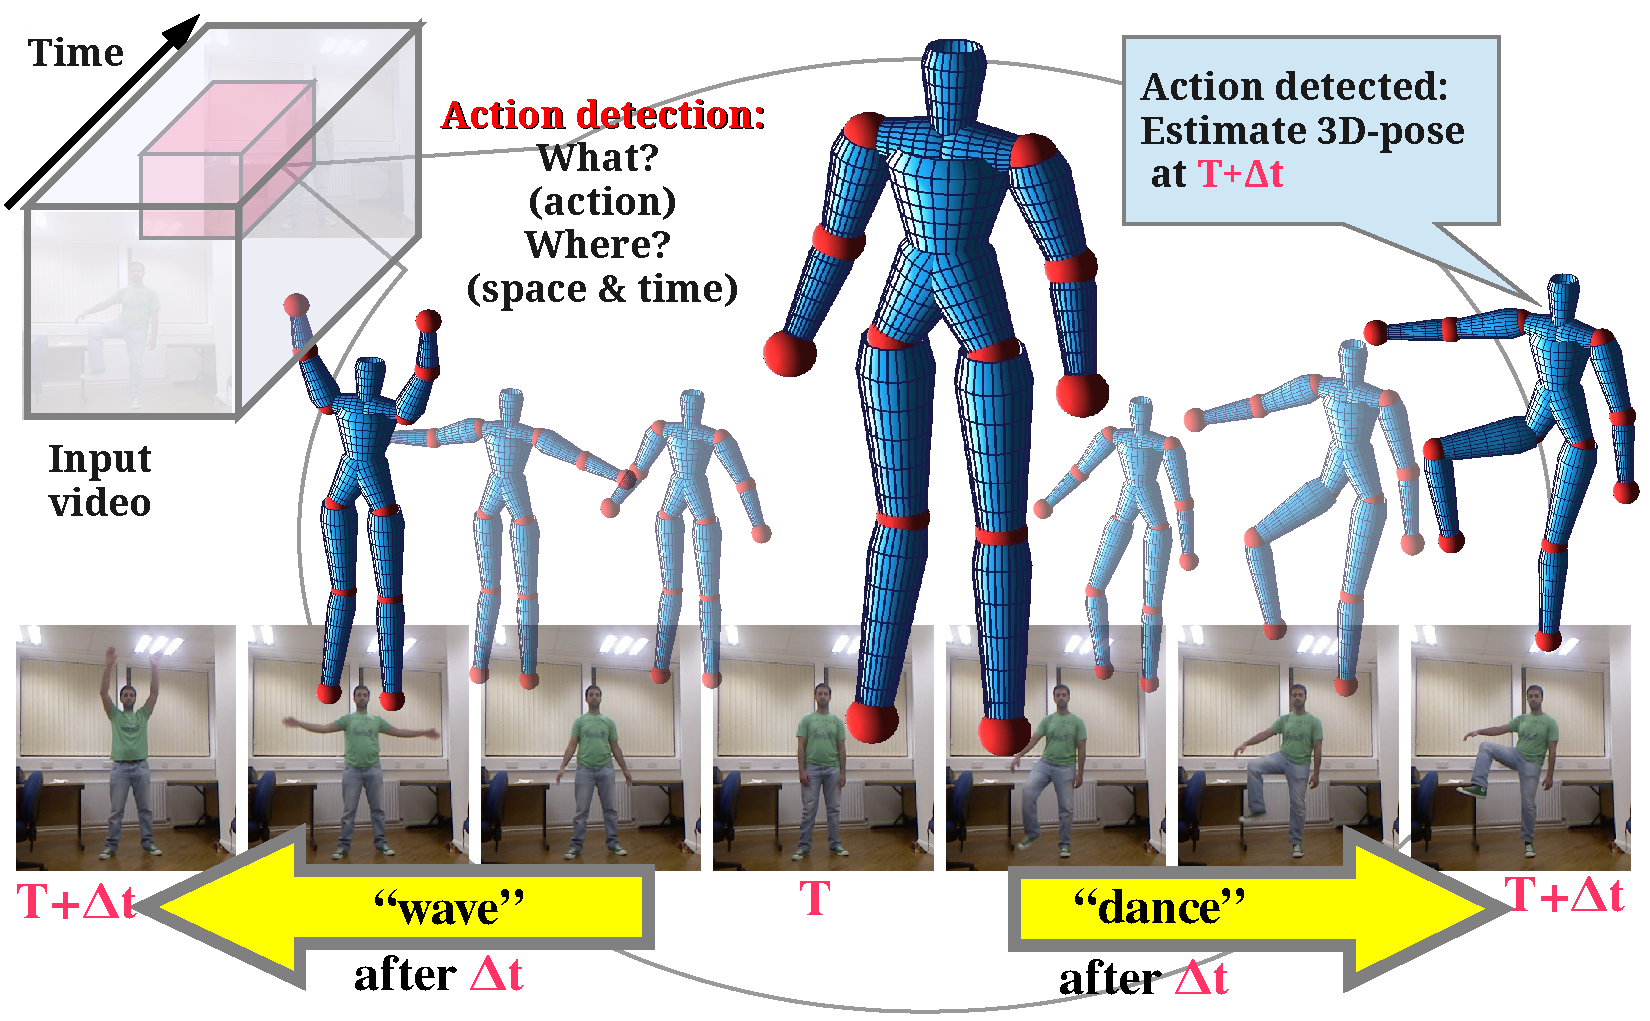
\includegraphics[width=1\linewidth]{fig/body/figure1_actionexplain.pdf} 
	\caption{Action detection helps 3D pose estimation by providing the spatiotemporal structure of actions.} 
	\label{fig/body/actionexplain}
\end{figure}

\begin{figure}[ht]
	\centering
	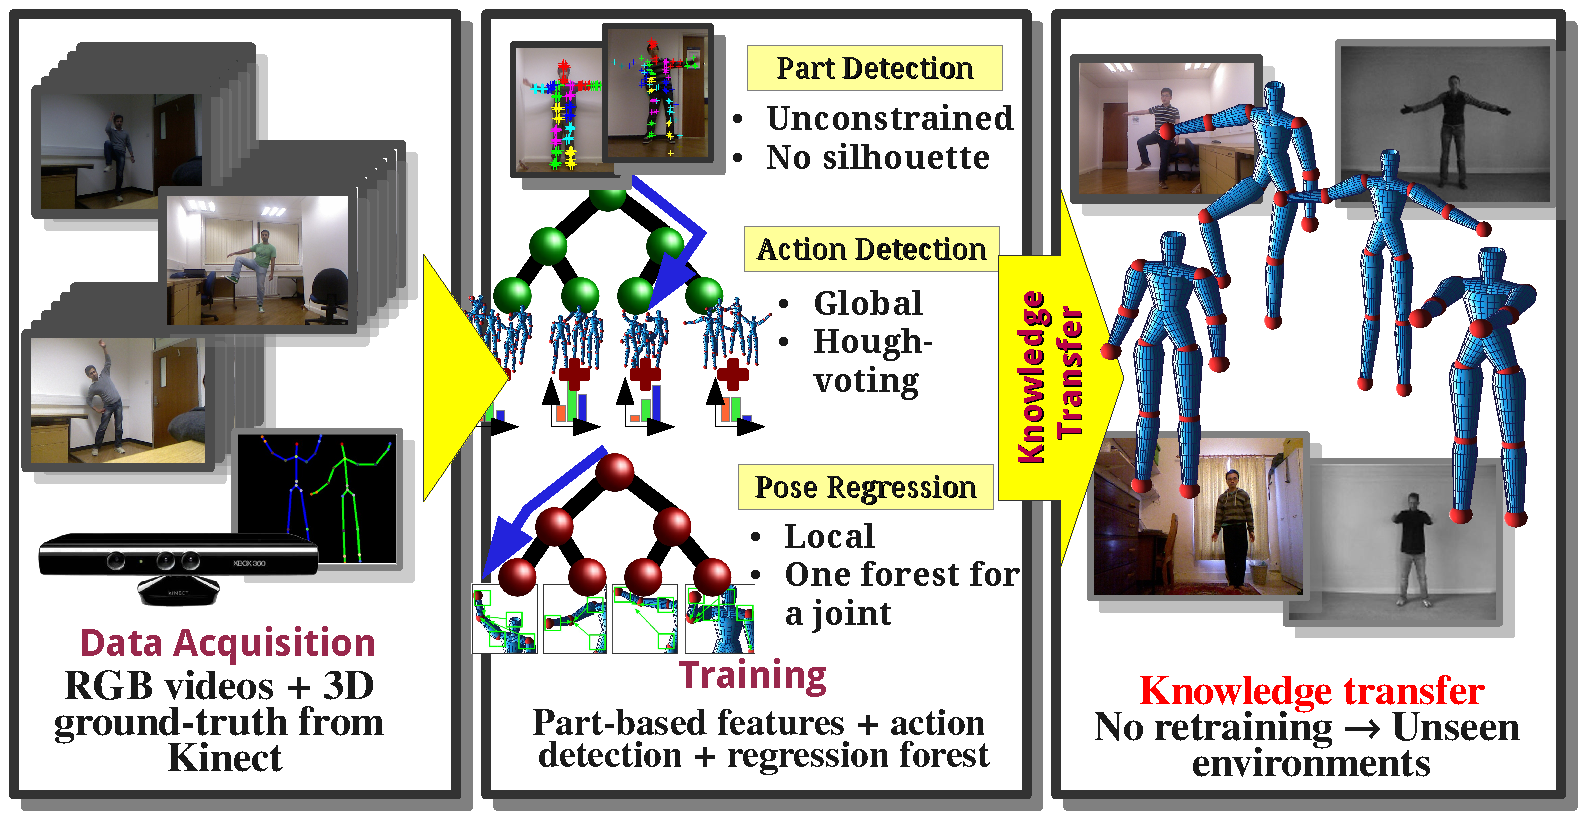
\includegraphics[width=1\linewidth]{fig/body/figure2_transferexplain.pdf}
	\caption{Knowledge transfer capability of the proposed method} 
	\label{fig/body/transferexplain}
\end{figure}

%------------- backup 
%\begin{figure}[ht]
%	\centering
%	\includegraphics[width=1\linewidth]{fig/body/actionexplain.pdf}
%	\caption{Action detection helps 3D pose estimation by providing the spatiotemporal structure of actions.} 
%	\label{fig/body/actionexplain}
%\end{figure}
%-------------backup end

%\subsection{Motivations}
3D human pose estimation (HPE) has been a longstanding challenge in computer vision.
3D HPE aims to infer a human pose, represented by joint positions or angles, from input images or videos.  
%Articulated body pose estimation has been a longstanding problem in computer vision with various applications such as video analysis, motion capture and surveillance.
% what is 3D HPE? Do we need to explain that?  
Contemporary methods commonly approach 3D pose estimation as a regression or a manifold learning scenario, features are embedded to a parametrised 3D pose space. 
%, poses are estimated by learning a mapping is learnt from the appearance space to the 3D pose space. 
However, learning mappings between high-dimensional spaces is an essentially ill-posed problem \cite{Elgammal2004}. Additional priors are needed to optimise a correct pose from multiple hypotheses. 
These priors are crucial to pose estimation, however, they also require a much controlled environment to capture compatible data: clean background segmentation, a calibrated multi-camera network, and depth sensor. 
Furthermore, if there are changes to the imaging environment, the whole pose estimator has to be retrained, making the pose estimation algorithm not scalable. 
%Furthermore, the pose estimator has to be retrained if the imaging environment changes, making the pose estimation algorithm not scalable.  

%including multi-view videos, body segmentation and specialized hardware. 
%Ideal imaging conditions, such as a clean background and calibrated camera system, seldom exist in realistic applications. 

%\begin{figure}[ht]
%	\centering
%	\includegraphics[width=1\linewidth]{fig/body/transferexplain.pdf}
%	\caption{Knowledge transfer capability of the proposed method} 
%	\label{fig/body/transferexplain}
%\end{figure}
In this chapter, we present a new method that incorporates action detection and 2D part-based pose estimation techniques for realistic, video-based 3D pose estimation. Our contributions are three-folds: 
\paragraph{Action detection.} Firstly, we combine action detection with 3D pose estimation to utilise the strong spatiotemporal structures of actions.
The analysis of human pose and action are two closely interrelated areas in computer vision. Although there exist initial studies in using human poses for recognising actions \eg \cite{Yao2012, Wang2012}, the opposite direction, \ie using actions to help pose analysis, 
is still an aspect that many methods have overlooked. 
An atomic action is considered as a time series of poses, with particular starting/ending poses and their transitions in-between. By detecting an atomic action in video,  a strong 3D pose prior per each frame is obtained. 
%in pose estimation. 
%In computer vision, learning pose and action are two closely interrelated areas.
%, 3D poses can be estimated by transferring the knowledge learned from action. 
%However, the temporal structures of human poses is an aspect that many methods have overlooked. 
In addition to kinematic constraints, action determines the temporal structure of a series of poses. For instance, in figure \ref{fig/body/actionexplain}, action detection simultaneously estimates the action category and the space-time location of an action, supporting pose estimation within the action's time span.
%estimates both the category and temporal location of an action. are detected from input video snippets, giving a strong prior for pose estimation. Besides recognising action categories, an action detector also estimates the temporal location of an action, providing a respecitve pose hypothsis per frame.  
%We therefore propose action detection in video as a strong resonable prior for 3D pose estimation.
\paragraph{2D part detection.} Secondly, we apply 2D part-based pose estimation techniques to infer 3D articulated poses. 
Holistic shape features, such as silhouettes which rely on background segmentation, are replaced by a deformable part model (DPM), \eg \cite{Yang2011}, to maximise flexibility. Our method is therefore knowledge transferable, learned models can be reused in unseen environments without retraining (see figure~\ref{fig/body/transferexplain}). 
\paragraph{Cross-modality regression forest.} 
Finally, we refine 3D human poses from 2D part detections using cross-modality regression forests.
To the best of our knowledge, this is the first application of regression forest~\cite{Criminisi2011} across modalities to 3D HPE problem.  
Estimating 3D human pose is essentially a cross-modality regression problem: 
\emph{3D structure} of a human pose is inferred using features extracted from its \emph{2D appearance} 
%Learning a regression across the two modalities is difficult, because the relationship between them are implicit.
Since the relationship between the two spaces are implicit, learning a robust regression model across two modalities becomes a challenging issue. 
The regression forests estimate joint positions in 3D from detected 2D parts, which are combined with action detection to optimise 3D pose estimation. 
The outputs of both forests, and their combined results, are formulated in a probabilistic framework. 
While some methods yield a point estimate in the pose space, our approach outputs joint positions as probability distributions in 3D space. 
%We design a algorithm to refine 3D joint positions using cross-modality regression forest. 
% 3D joint positions are refined, from detected 2D parts and action categories, using a cross-modality regression forest. 

%The rest of the paper is organised as follows: 
%relevant work is reviewed in section \ref{sec/body/review}. 
%The proposed method is detailed in section \ref{sec/body/method}. Section \ref{sec/body/eval} describes the experimental framework and performance evaluation. Finally, section \ref{sec/body/conclusions} concludes with discussions and furture work. 

\section{Literature Review}
\label{sec/body/review}

\paragraph{Early methods.} 
Part-based 2D pose analysis has been studied for decades, examples of early approaches include \eg pictorial structure \cite{Fischler1973} and template matching \cite{Ioffe1999}. 
However, these methods are limited due to the lack of an automatic part detector, which implies manual labelling required for both training and testing data. 
%However, these methods are greatly limited as they require manuall labeled data.
3D human pose estimation is more complicated than its 2D counterpart due to occlusions and high dimensionality. 
To estimate 3D pose from video data, various techniques have been proposed, \eg image edges \cite{Hogg1983} and silhouettes \cite{Navaratnam2006}. Approaches for traditional 3D human pose estimation are discussed in \cite{Poppe2007}. 
Cross-modality approach had not been explored until \cite{Micilotta2006}, where 2D face and hand detectors were used to infer a simple 3D pose of upper body.  

%The spatial arrangements of body parts have been widely used in 2D human pose anaylsis. For example, Fischler and Elschlager \cite{Fischler1973} conceptualized \emph{pictorial structure} for modeling the spatial structure of human pose, Ioffe et al. \cite{IOffe1999} described body parts as a collection of image templates. 
%However, the effectiveness of these approaches were greatly limited due to the lack of robust detectors for different body parts, manual labelling of body parts was often required. 
%On the other hand, 3D pose estimation is more complicated than its 2D counterpart, due to occlusions and a high dimensionality in the pose space. Various methods have been developed: Hogg \cite{Hogg1983} used image edges to compute the 3D pose of a walking person from a carefully controlled environment. 
%Micilotta et al. \cite{Micilotta2006} used several part detectors, e.g. face and hand detectors, to infer a simple 3D pose of the person upper body. A regression algorithm was presented by Navaratnam et al. \cite{Navaratnam2006} to compute 3D poses from silhouettes. 
%\subsubsection{Recent approaches}

More recent techniques of human pose estimation are discussed below according to the techniques or representations used.

\paragraph{Silhouette or depth image.} 
Holistic shapes, silhouettes in particular, are common features for 3D pose estimation. 
Current approaches achieve state-of-the-art performance by combining silhouettes with new features or constraints, including motion templates \cite{Rogez2012}, pedestrian detectors \cite{Andriluka2010}, shape-contents \cite{Agarwal2006} and user interaction \cite{Guan2009}.  
%State-of-the-art performances are achieved by combining silhouettes with new features or constraints, including motion templates \cite{Rogez2012}, pedestrian detector \cite{Andriluka2010}, shape-context \cite{Agarwal2006} and user interaction \cite{Guan2009}.  
Thanks to the introduction of the Kinect sensor, using depth images emerges as a new direction for 3D HPE, as it provides inherent depth information and object segmentation. 
%Recently, several depth-based 3D HPE approaches have been introduced, such as \cite{Baak2011}, \cite{Ye2011} and \cite{Sun2012}. 
Several methods recognise 3D human poses from depth images, using techniques such as point cloud matching \cite{Baak2011, Ye2011} and random forest \cite{Taylor2012, Sun2012}. 
However, many of the above methods require an accurate image segmentation to extract shape features, thus special hardware (\eg Kinect sensor) or controlled environments are often necessary to acquire compatible training or testing data.  
%for the task.
%For instance, Bissacco et al. \cite{Bissacco2007} proposed a boosting classifier to compute human poses from both silhouettes and motion features.  
%Guan et al. \cite{Guan2009} estimated human poses and shapes simultaneously from silhouettes, assisted by manual initializations.
%A lantent structured model is described in \cite{Ionescu2011} to estimate 3D poses from silhouettes. 
%Pons et al. \cite{Pons-Moll2011} presented a pose optimization algorithm from silhouettes captured from multiple cameras. 
%Motion templates are also used in 3D pose estimation, \cite{Rogez2012} used a global motion template to recognize poses using a tree-shape ensemble of rejectors. 
%Recently, depth sensor has become a popular imaging technique for computer vision as it provides inherent depth information as well as object segmentation.  
%Several methods are proposed to estimate 3D human poses from depth images, using techniques such as point cloud matching \cite{Baak2011, Ye2011} and random forest \cite{Sun2012}. 
%However, many of these methods on both silhouette and depth require an accurate segmentation to extract shape features from input data, thus specialized hardware and unconstrained environments are often required. 

\paragraph{Multiple-cameras.} 
A common approach to resolve the pose ambiguity is to maximise the field of view by capturing multiple images simultaneously using calibrated cameras, \eg \cite{Pons-Moll2011, Sigal2012, Yao2012}. Although they achieve excellent accuracy, potential applications are restricted to a fixed, calibrated multi-camera system. 
%Resolving the pose ambiguity from multiple views is, still, a sophisicated optimization problem. Existing solutions are often computationally expensive, which further limits its applicability.   
%
%{\bf Multiple-cameras.}
%A common approach to resolve the pose ambiguity, caused by the limitation of 2D image-baed features, is to capture several images simultaneously using multiple calibrated cameras, such as 
%\cite{Pons-Moll2011, Sigal2012, Yao2012}. Accoridingly, it restricts potential applications to a fixed, calibrated multi-camera system. Furthermore, resolving the pose ambiguity from multiple views is, still, a sophisicated optimization problem. Existing solutions are often computationally expensive, which further limits its applicability.   
% Pose ambiguity is a common issue for 3D pose estimation.
%%Due to the limitation of 2D, image-based features, multiple solutions of 3D poses can be found in one estimation.
\paragraph{Action for pose estimation.}
As mentioned previously, the integration of action and pose, in particular action for pose, is still a largely unexplored area. We seek to investigate the feasibility of using \emph{action detection} to facilitate 3D human pose estimation in uncontrolled and monocular videos.
Early approaches that combines action and pose constrains include \cite{Yu2010} and \cite{Raja2011}.
The closest work to this idea is \cite{Yao2012} that uses action recognition to assist a multi-view 3D HPE algorithm. Separate regression models are trained; After an action is recognised, poses are inferred using the model of the action class estimated. 
Whilst action recognition is applied, the inputs are still images captured from a controlled, multi-camera environment. 
Instead, we perform action detection in video, by which we exploit the spatiotemporal structure of actions in addition to action class labels, to infer 3D poses.
%When the action of a person is detected in a video, it gives much information about spatiotemporal structure of that person, which is extrmely useful in the pose estimation task.  
%For instance, when a ``walking'' action is detected, it gives a strong \emph{spatial} prior to the pose estimator as outputs are limited to the ``walking'' poses. 
% However, the combination of pose estimation and action detection techniques is still a largely unexplored area. 
% \emph{temporal} used is obtained to support the pose estimator. 
%By tracing the current pose from the starting time of the action detected,
%Action recognition is performed by single images, action category labels are only used as a switch to different manifolds, where the 3D poses are estimated. 
%in uncontrolled single video. 
%a main object of our model is to estimate s by leveraging 
%has not utilized the inherit spatiotemporal structure of an \emph{action}--

\begin{figure}[ht]
	\centering
	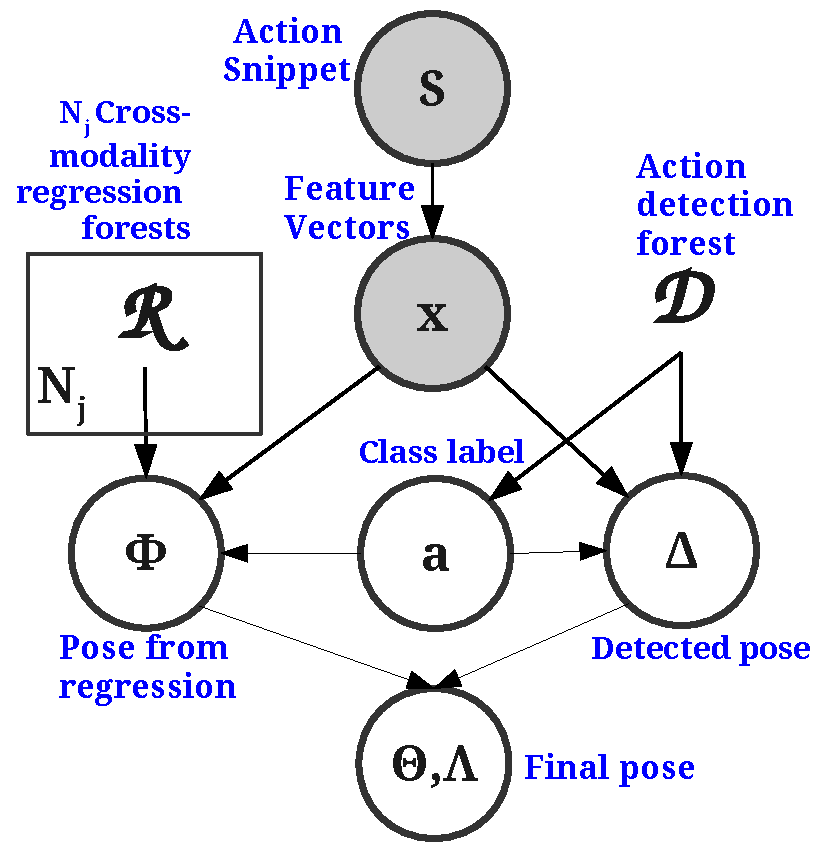
\includegraphics[width=0.35\linewidth]{fig/body/figure4.pdf}
	\caption{Graphical representation of the proposed model} 
	\label{fig/body/figure4gm}
\end{figure}

\begin{figure}[ht]
	\centering
	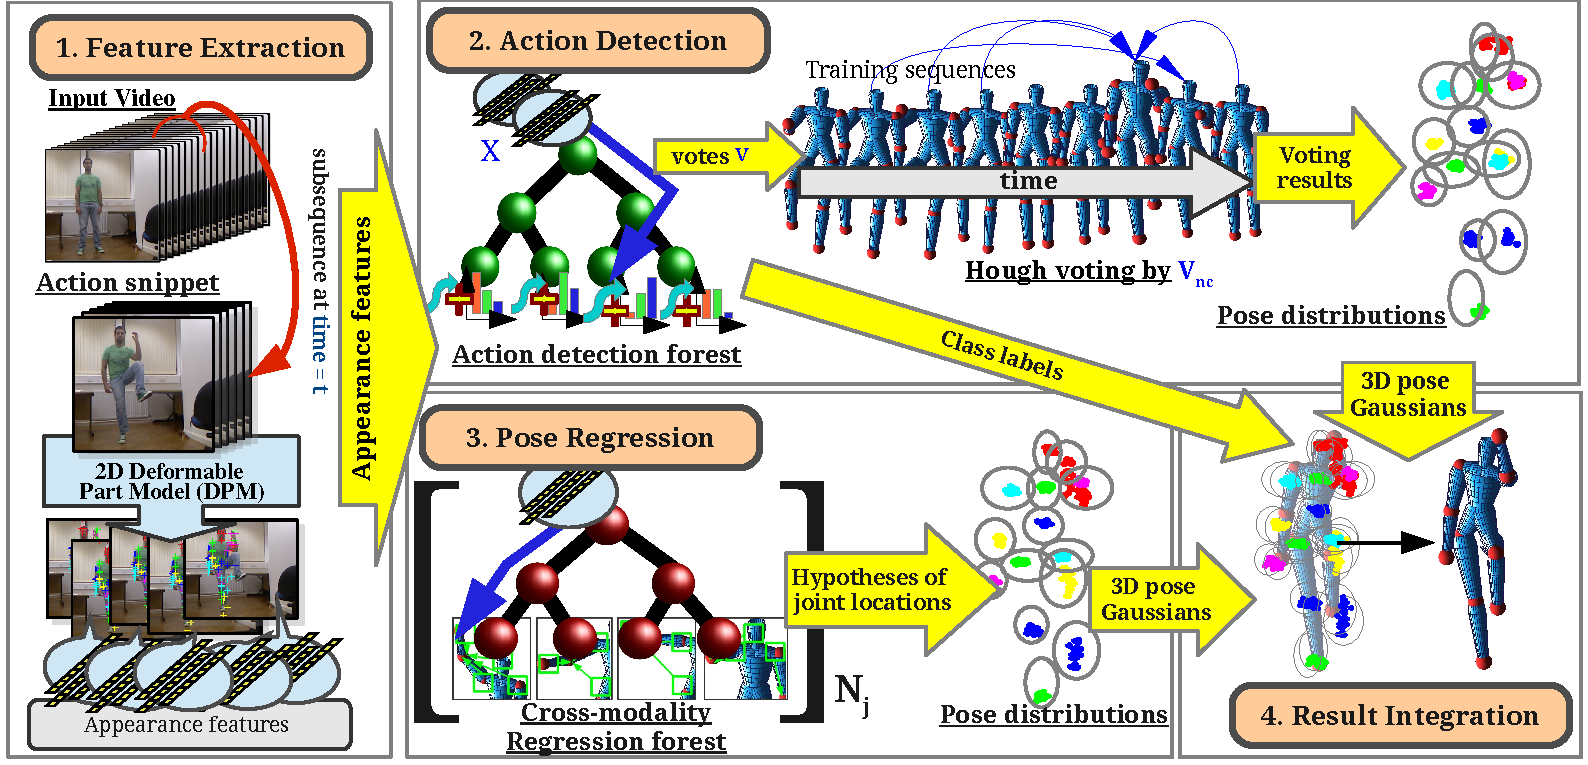
\includegraphics[width=1\linewidth]{fig/body/figure3_overview.pdf}
	\caption{Overview of the proposed framework}
	\label{fig/body/overview}
\end{figure} 

\paragraph{Part-based pose estimation.} 
Various methods have been introduced built upon the original seminal model of pictorial structures \cite{Felzenszwalb2000, Felzenszwalb2010}. Recent extensions include new motion features \cite{Andriluka2009}, improved part-based model learning and inference \cite{Yang2011, Sun2012a}, and pre-processing techniques (\eg face detector) \cite{Eichner2012}. 

%Current state-of-the-arts usually build upon the success of traditional methods with new features or improved models. For instance, Sapp et al. \cite{Sapp2011} modelled pictorial structure in a more complicated graph by decomposing the it into smaller, stretchable components. 
% Similarly, an branch-and-bound algorithm was proposed in \cite{Sun2012a} to extend traditional pictorial structure beyond star-shaped or tree graphs. 
% using new features 
%In \cite{Hua2007}, visual tracking is combined with part detection in order to estimate articulated human pose. 
%Ardriluka et al. \cite{Andriluka2009} revisited traditional pictorial structure using dense shape context and adaboost algorithm. 
%Eichner et al. \cite{Eichner2012} presented a multi-phase algorithm to detect 2D body parts from unconstrained images using various clues such as face detection and graph cut algorithm. 

%Despite achieving remarkable performances, particularly in uncontrolled environments, 
%As  has shown a better performance than its 3D counterpart, especially in uncontrolled environments, it is suggested that similar techniques can be applied %to improve 3D pose estimation results. As a result, recent advances in 2D pose estimation, e.g. deformable part-based models %\cite{Felzenszwalb2010}, inspired a resurgence of part-based approaches for 3D human pose estimation.   
Recent advances in 2D human pose estimation methods, particularly in uncontrolled environments, have inspired a resurgence of part-based approaches for 3D pose estimation. 
While some approaches use manually labelled 2D parts to estimate 3D poses, \eg \cite{Wei2009, Ramakrishna2012}, 
%the poselet algorithm \cite{Bourdev2009} estimate a rough 3D pose by learning 2D part templates. 
2D deformable part models are also investigated in 3D human pose estimation, for instance, \cite{Andriluka2010} uses a pedestrian detector with deformable body parts to estimate rough 3D poses in street scenes, 
\cite{Simo-Serra2012} optimises multiple pose hypotheses from 2D DPM using inverse kinematics to estimate 3D pose in a single image.
In this work, we further investigate the use of 2D DPM in a multi-action 3D HPE scenario. 

%Consequently, multi-action 3D pose estimation with deformable part model is a topic of great research potential. 
%Simo-Serra et al. \cite{Simoserra2012} estimate 3D poses in an image using multiple hypotheses obtained from a 2D pictorial structure model. 
%In addition, part-based models are also used to infer poses of walking pedestrians in videos\cite{Andriluka2010}. Meanwhile, the poselet algorithm \cite{Bourdev2009} uses templates of body parts to estimate a rough 3D pose from an unconstrained image. The above part-based approaches demonstrate a greater flexibility than holistic-based methods. Hence, part-based 3D pose estimation in a multi-action scenario has become a topic with great research potential. 

%By applying suitable inverse kinematics constraints, 3D poses can be estimated accurately from images with manually labeled parts \cite{Wei2009, RamakrishnaECCV2012}. 
%Simo-Serra et al. \cite{Simoserra2012} estimate 3D poses in an image using multiple hypotheses obtained from a 2D pictorial structure model. In addition, part-based models are also used to infer poses of walking pedestrians in videos\cite{Andriluka2010}. Meanwhile, the poselet algorithm \cite{Bourdev2009} uses templates of body parts to estimate a rough 3D pose from an unconstrained image. The above part-based approaches demonstrate a greater flexibility than holistic-based methods. Hence, part-based 3D pose estimation in a multi-action scenario has become a topic with great research potential. 
\section{Method}
\label{sec/body/method}

Figure \ref{fig/body/figure4gm} describes the graphical model of our 3D human pose estimation framework: action detection is performed to yield the rough 3D pose estimates, then cross-modality regression forests with the estimated action classes are applied to refine the 3D pose estimations. While full poses, \ie 3D coordinates of all $\njoints$ joints, are learnt in the action detection forest, one joint location is estimated per cross-modality regression forest. $\njoints$ regression forests are hence trained separately in the model. The conceptual data-flow of the proposed framework is illustrated in figure \ref{fig/body/overview}.

%used to refine
%After action detection, cross-modality regression forests are used to refine the rough 3D pose estimations given by the action detection process. 

\subsection{Part-based Feature Extraction}

In order to perform 3D pose estimation in different backgrounds and scenarios, input features are extracted using a 2D part-based model. 
Firstly, a deformable part model (DPM) \cite{Yang2011} is employed as an off-the-shelf method to extract body parts from input frames.
Unlike the traditional holistic silhouette-based methods, where background subtraction is preformed, our method based on body parts works at unseen and dynamic backgrounds. 
The DPM fires $\nhyp$ body part configurations per frame, each hypothesis contains $26$ locations of detected body parts as in \cite{Yang2011}. 
%hypotheses on configuration of $26$ body parts are obained per frame (the number of hypothese is dentoed ${\nhyp}$). 
Subsequently, the detected configurations are normalised with respect to the distance between the head and the waist part. 
Finally, a feature vector is computed per configuration by the pairwise distances among the normalised parts, hence the feature vector takes $325 (=26\times25/2)$ dimensions.

In the training process, every feature vector is associated with a ground truth 3D pose.
The Kinect sensor is used to acquire 3D poses simultaneously with the RGB video sequences. 
A 3D human pose is represented by the scale-normalised coordinates of the $\njoints$ joints detected by the Kinect sensor, an articulated model of $\njoints=15$ joints is used in this work. 
Every feature vector in the training dataset is assigned to the 3D pose detected and one of the $\nclass$ action categories, according to its corresponding frame and video. The feature vectors are denoted as $\fset = \{\feature_{\videoth\frameth\hypth}\}$, where $\feature_{\videoth\frameth\hypth}$ is the $\hypth$-th configuration detected in the $\frameth$-th frame of the $\videoth$-th training video. The corresponding class label and corresponding 3D pose
are defined as  $\aset = \{\action_{\videoth\frameth\hypth} | \action_{\videoth\frameth\hypth} \in 1,\dots,\nclass \}$ and $\pset = \{\bodypose_{\videoth\frameth\hypth} | \bodypose_{\videoth\frameth\hypth} \in \realnum^{3\njoints}\}$ respectively.  
Furthermore, 3D poses $\pset$ of each action category are compressed separately into low-dimensional vectors $\ppset = \{\_{\videoth\frameth\hypth}  | \pbodypose_{\videoth\frameth\hypth} \in \realnum^{\pcadim} \}$ using PCA. 

% in the $\frameth$-th frame of the $\videoth$-th video 






\subsection{Learning} 

\paragraph{Action Detection Forest.}
\label{sec/body/adflearn}
The action detection forest, $\forestd$, performs action categorisation and 3D pose clustering simultaneously. 
In each leaf node, the 3D pose vectors $\ppset$ are classified into the action class labels $\aset$ and cohering 3D pose vectors are grouped together.
For given data triplets $\fset$, $\ppset$ and $\aset$, we grow $\ntreed$ decision trees by recursively splitting the data into two child nodes, where candidate split functions are generated randomly, each compares a value in the feature vector $\feature$ with a threshold. The best split is chosen among the candidates by maximising a quality measure. The splitting process is performed until the new node reaches its maximum depth or minimum number of data points. Lastly, every leave node stores the votes that are required in Hough-voting for action detection during testing. 

%are grouped coherent to form a 3D pose cluster. 

%is essentially a Hough forest \cite{Gall2011}, where,

%use to classify parts and let parts vote for the center of atomatic actions in space and time. 
%hybrid of clssification and clustering forest learnt using

%for object detection  with classification capability. 
%A decision tree is grown by passing down a random subset of training data from the root node. 
%Candidate split functions are generated randomly, each compares a feature value with a threshold. 
%n a new node, the optimal split is chosen among the candidates by maximizing a quality measure. 
%Incoming training data are divided into two subsets, which are passed down to two new child nodes.  

%Both classification and detection are performed in a single decision tree. To this end,

We propose a new integrated quality measure $\qualityad(\cdot)$ at the node $\curnode$ as:
%is proposed in equation \ref{eq:newquality}:
%\begin{align}
%	\label{eq:newquality}
%	\qualityad(\ppset_{\curnode}) & = \alpha \infogain(\ppset_{\curnode}) + (1-\alpha)\qualityjr(\ppset_{\curnode}) \\ 
%	\qualityjr(\ppset_{\curnode}) & = \displaystyle\sum_{c = 1}^{\nclass} \Psi(\Sigma(\ppset_{\curnode c})) - \nodeweight_{L}\Psi(\Sigma(\ppset_{Lc})) - \nodeweight_{R}\Psi(\Sigma(\ppset_{Rc}))\\
%	\alpha & = \max_{c}(|\aset_{\curnode} = c| / |\aset-{\curnode}|)- \min_{c} (|\aset_\curnode = c| / | \aset_{\curnode}|)
%\end{align}
\begin{align}
	\label{eq:newquality}
	\qualityad(\ppset_{\curnode}) & = (1 - \omega)\infogain(\ppset_{\curnode}) + \omega\qualityjr(\ppset_{\curnode}). 
\end{align}
The first term, $\infogain(\cdot)$, is the information gain measure used in standard classification forest \cite{Breiman2001} (here for action classification); the second term measures the improvement in 3D pose coherence when a split is performed    
\begin{equation}
	\qualityjr(\ppset_{\curnode}) = \displaystyle\sum_{c = 1}^{\nclass} \Psi(\Sigma(\ppset_{\curnode c})) - \Psi(\Sigma(\ppset_{lc})) 
- \Psi(\Sigma(\ppset_{rc})),
\end{equation} 
where $\Psi(\cdot) = \log(\det(\cdot)) $ and $\Sigma(\ppset_{\curnode c})$ is the covariance matrix of the PCA-compressed 3D pose vectors  $\ppset_{\curnode c}$ of the n-th node ($l,r$ denote the left and right split respectively) and the $c$-th action class. These measures are weighted by $\omega$ that describes the class purity of a node as
\begin{equation}
	\omega = \max_{c}(|\aset_{\curnode c}| / |\aset_{\curnode}|)- \min_{c} (|\aset_{\curnode c}| / | \aset_{\curnode}|),
\end{equation} 
where $\aset_{\curnode}$ denotes the action labels of training data in node $\curnode$ and $\aset_{\curnode c}$ the action labels of node $\curnode$ and class $c$. The first quality term in (\ref{eq:newquality})  optimises action classification performance while the second term optimises pose clustering performance within a node. Initially, classification is preferred over clustering, $\infogain(\cdot)$ is dominant when class labels are evenly distributed. However, $\omega$ gradually increases as the tree grows, shifting the learning focus to clustering. 

%$\aset_{\curnode c} = \{\action_{\curnode} = c| \action_{\curnode} \in \aset_{\curnode}\}$. 

%Information gain $\infogain$ \cite{Breiman2001} is applied initially to optimize classification performance. When class entropy decreases in deeper nodes, e.g. more than $90\%$ of the training instances belong to the same label, the second quality measure $\qualityad$ is used instead to optimize for detection accuracy: 
%where $\ppset_{\curnode c}$ represents the training dataset in current node $\curnode$ with class label $c$, it is split into two subsets 
%$\ppset_{Lc}$ and $\ppset_{Rc}$ to the left and right child nodes. 
%The compactness of 3D poses in a node is measured by the log-determinant of covariance $\log|\Sigma(\cdot)|$. 
%The quality measure is the increase in node data compactness after the split, weighted by the node size ratio $\nodeweight_{L} = |\ppset^{\curnode}_{Lc}| / |\ppset_{\curnode c}|$ and $\nodeweight_{R} = 1 - \nodeweight_{L}$.

% a small subset of data remains in each leaf node.
Once the learning is completed, the class posterior of a leaf node $\termnode$ is obtained by:  
\begin{equation}
	\label{eq:dforest_treeposterior}
	P(\action = c| \termnode) = |\aset_{\termnode c}|/| \aset_{\termnode}| 
\end{equation}
The distribution of 3D poses, given a action class-label $c$, is modelled by a Gaussian 
$\normdist(\mu({\ppset}_{\termnode c}), \Sigma(\ppset_{\termnode c}))$.
A vote $\vote_{\termnode c}$ cast by the leaf node is a  pair  
$ \vote_{\termnode c}= ( \videoth_{\termnode c}, \frameth_{\termnode c}), c = 1,...,\nclass$ such that
\begin{equation}
	(\videoth_{\termnode c}, \frameth_{\termnode c}) =  
	\displaystyle\argmin_{(\videoth, \frameth)} || \_{\videoth\frameth\hypth} - \mu({\ppset}_{\termnode c}) ||_{2}
\end{equation}
$\videoth_{\termnode c}$ and $\frameth_{\termnode c}$ are the indices of the training sample that is the nearest neighbour of Gaussian mean $\mu(\ppset_{\termnode c})$. As a result, $\frameth$ is a temporal vote to the staring point of actions in sequence $\videoth$.

% = \sum_{i}^{|\ppset_{\termnode c}|} \ppset_{\termnode c i}/|\ppset_{\termnode c}|$.


%back-projected 3D poses of the above Gaussian means, such that:
%where the mean is approximated by its nearest neighbour in the training dataset.  


%\begin{equation}
%	\begin{array}{c}
%
%		\videoth_{c\termnode}, \frameth_{c\termnode}, \hypth_{c\termnode} =  
%		\displaystyle\argmin_{\videoth, \frameth, \hypth} || \_{\videoth\frameth\hypth} - \overline{\ppset}_{\termnode} ||_{2}  \\
%
%		P(\'| \termnode, \action_{\termnode} = c) = \normdist(\pbodypose',%\pbodypose_{\videoth_{c\termnode}\frameth_{c\termnode}\hypth_{c\termnode}},  \Sigma(\ppset_{c\termnode})) 
%
%	\end{array}
%\end{equation}


%\begin{figure}[ht]
%\begin{center}
%\vspace{5cm}
% %\includegraphics[width=0.8\linewidth]{egfigure.eps}
%\end{center}
%   \caption{Methods in details.}
%\label{fig/body/long}
%\end{figure*}

\paragraph{Cross-modality Regression Forest.}
\label{sec:jrflearn}
The cross-modality regression forests $\{\forestr^{(j)}|{j} = 1,\dots,\njoints\}$, inspired by \cite{Criminisi2011}, are learned to refine the 3D locations of joints. Each forest $\forestr^{(j)}$ contains $\ntreer$ trees that estimate the location of the $j$-th joint, trained independely from the dataset $\{ \pset^{(j)}, \fset, \aset\}$, where $\pset^{(j)}$ is the $j$-th joint's 3D coordinates in $\pset$. 
Split function candidates are generated in the same way as action detection using the feature vector $\feature$. 
%We assume that class esimates are given during testing by the detection forest, so . 
Although action class posteriors can be computed in the terminal nodes, it is not modelled in this method as the action detection forest $\forestd$ provides a better action recognition rate that helps the localisation accuracies of $\forestr^{(j)}$. Thus, $\qualityjr(\pset^{(j)}_{\curnode})$ is used instead to optimise the split functions for the localisation accuracy of the $j$-th joint. 
% ---- back up 
%\begin{equation}
	% \qualityjr(\pset^{(m)}_{\curnode c}) = \displaystyle\sum_{c = 1}^{\nclass} \left(  \log|\Sigma(\pset^{(m)}_{\curnode c})| - \nodeweight_{L}\log|\Sigma(\pset^{(y)}_{Lc})| - \nodeweight_{R}\log|\Sigma(\pset^{(m)}_{Rc})| \right)
%	\qualityjr(\pset^{(m)}_{\curnode}) = \displaystyle\sum_{c = 1}^{\nclass} \Psi(\Sigma(\pset_{\curnode c})) - %\nodeweight_{L}\Psi(\Sigma(\pset_{Lc})) - \nodeweight_{R}\Psi(\Sigma(\pset_{Rc}))
%\end{equation}
% ---- back up

% not neccessary
% where $\pset^{(m)}_{\curnode c}$, $\pset^{(m)}_{L c}$ and $\pset^{(m)}_{R c}$ are the training data in $\curnode$, its left child and right child respectively. 
% Since the action class labels are recognized in advanced via action detection, the quality function $\qualityjr$ aims to minimize the uncertainty in joint regression rather than classification error.
Tree growing is stopped when the current node is smaller than a certain size.
Upon completion of $\forestr^{(j)}$, the output of its leaf nodes $\termnode$ are described by the mean joint coordinates with respect to class label, given by $\mu(\pset^{(j)}_{\termnode c})$.  

%The mean $\overline{\pset^{(m)}_{\termnode c}}$ is not computed for class $c$ no data is present in $\termnode$.  


\subsection{Testing}

Video snippet, the basic unit required for action detection \cite{Schindler2008}, is a short sequence excerpted from the testing video, centered at time $\timenow$. A snippet $\snippetnow$ contains $\snippetlen$ frames such that $\snippetnow = \left\{ \sframe_{\timenow - \snippetlen/2}, \dots, \sframe_{\timenow + \snippetlen/2 - 1} \right\}$. The testing process starts with extracting features from $\snippetnow$, such that $\fset_{\snippetnow} = \{ \feature_{ij}\}$, where $i =\timenow-\snippetlen/2,...,\timenow+\snippetlen/2-1$ and $j=1,...,\nhyp$ with $\nhyp$ denotes the number of part configurations of the frame.
\paragraph{Action detection (classification).} 
\label{sec:adftest}
Action detection forest $\forestd$ performs action classification on $\snippetnow$. Let $\termnode_k[\feature_{ij}]$ be the leaf node reached by a feature $\feature_{ij}$ in the $k$-th tree of $\forestd$. The posterior of snippet action class at time $t$ is defined as 
\begin{equation}
	P(\action = c | \snippetnow, \forestd) = \sum_{k,i,j = 1}^{\ntreed, l, \nhyp}\frac {P(\action=c|\termnode_{k}[\feature_{ij}])} {\ntreed l \nhyp}. 
\end{equation} 
%Consequently, the pose found in $\sframe_{\timenow}$ can be estimated from $\snippetnow$ by action detection. 
\paragraph{Action detection (pose voting).}
A Hough-based voting scheme is designed for action detection. 
As mentioned in section \ref{sec/body/adflearn}, the vote $(p,q)$ stored in $\forestd$ are temporally associated with their corresponding action sequence and time frame in the training data set. Note each training frame is paired with a ground truth 3D pose. Hence, all frames $I$ can vote for a 3D pose at time $\timenow$, by applying temporal offsets  $\delta$ to the votes obtained from $\fset_{\snippetnow}$. We define a function $\Delta(\snippetnow,c)$ that returns a set of 3D pose estimates in $\pset$ for action label $c$ from Hough-voting during action detection: 
%The set of votes $\vset[\sframe_i] = \{ \videoth_{k c}[\sframe_{i}], \frameth_{k c}[\sframe_{i}]|k\!\in\!1,\dots,\nvset;c\!\in\!1,\dots,\nclass\}$ is obtained by passing down $\forestd$ the features extracted form a frame in snippet $\sframe_{i} \in \snippetnow$. 
\begin{equation}
	\Delta(\snippetnow, c) = \pset^{\Delta}_{\termnode_{k}[\feature_{(t+\delta)j}]c}
\end{equation}
where $ k = 1,...,\ntreed$, $\delta = -\snippetlen/2,...,\snippetlen/2-1$, $j = 1,...,\nhyp$. The set $\pset^{\Delta}_{\termnode_{k}[\feature_{(t+\delta)j}]c}$ denotes the $\delta$-voted (offset-ed) pose from the $\delta$-th frame in $\snippetnow$, \ie $(t\!+\!\delta)$-th frame in input video, by passing down the $k$-th tree in $\forestd$
%are the poses associated with the votes obtained from $\snippetnow$, such that
\begin{equation}
	\begin{split}
		& \pset^{\Delta}_{\termnode_{k}[\feature_{(t+\delta)j}]c} = \{\bodypose_{\videoth(\frameth-\delta)\hypth}\}\\ 
		\mbox{ s.t. } & (\videoth,\frameth) = \vote_{\termnode_{k}[\feature_{(t+\delta)j}]c} \mbox{ and } \action_{\videoth\frameth\hypth} = c 
\end{split} 
\end{equation} 

% ----------------- BACK UP 2
%\begin{equation}
%\pset^{\mathcal{D}}_{c} = \{ \bodypose^{\Delta}_{\termnode_{k}[\feature_{(t+\delta)j}]c}\}
%\end{equation}
%where $j = [1,\nhyp]$, $\delta = [-\snippetlen/2,\snippetlen/2]$,  $ k = [1,\ntreed]$. The set $\bodypose^{\Delta}_{\termnode_{k}[\feature_{(t+\delta)j}]c}$ denotes the $\delta$-voted (offseted) pose from the $\delta$-th frame in $\snippetnow$, \ie $(t\!+\!\delta)$-th frame in input video, by passing down the $k$-th tree in $\forestd$
%are the poses associated with the votes obtained from $\snippetnow$, such that
%\begin{equation}
%	\begin{split}
%		& \bodypose^{\Delta}_{\termnode_{k}[\feature_{(t+\delta)j}]c} = \bodypose_{\videoth(\frameth-\delta)\hypth}\\ 
%		\mbox{ s.t. } & \videoth,\frameth\in\vote_{\termnode_{k}[\feature_{(t+\delta)j}]c}, \aset_{\videoth} = c 
%\end{split} 
%\end{equation} 
%------------------ BACK UP 1
%\begin{equation}
%	\end{
%The set of all votes cast by $\snippet_\timenow$, in the 3D pose space is defined in equation \ref{eq:allDetectVotes}:
%\begin{equation}
%	\label{eq:allDetectVotes}
%	\begin{aligned}[lcl]
%		\vset_{\_{\timenow c}} & = & \{\vset^{-\delta}_{\termnode[\sframe_{t + \delta}]};\; \delta \in [-\timenow/2,\timenow/2 )\} \\
%		\vset^{-\delta}_{\termnode[\sframe_{t + \delta}]} & = & \{\bodypose_{\videoth_{c\termnode}\frameth_{c(\termnode-i)}\hypth_{c\termnode}}; \; c = i, \dots, \nclass \}
%	\end{aligned} 
%\end{equation}
Elements returned from $\Delta(\snippetnow, c)$ represent 3D pose estimations at time $\timenow$. A 3D pose $\bodyposead_{\timenow}$ is hence modelled by $\njoints$ independent Gaussians with respect to its joints. 
\begin{equation}
	\begin{split}
		& P( \bodyposead^{(j)}_{\timenow}| \snippetnow, \action = c,\forestd) \\ 
	 & = \normdist(\bodyposead^{(j)}_{\timenow}; \mu(\Delta^{(j)}(\snippetnow,c)), \Sigma(\Delta^{(j)}(\snippetnow,c))
\end{split} 
\end{equation}
where $\bodyposead_{\timenow}^{(j)}\in\realnum^{3}$ is the $j$-th joint in $\bodyposead_{\timenow}\in\realnum^{3\njoints}$.
% backup---------------------------
%\begin{equation}
%	\begin{split}
%		& P( \bodyposead^{(j)}_{\timenow}| \snippetnow, \action = c,\forestd) \\ 
%	 & = \normdist(\bodyposead^{(j)}_{\timenow}; \mu(\pset^{\mathcal{D}(j)}_{c}), \Sigma(\pset^{\mathcal{D}(j)}_{\timenow c}))
%\end{split} 
%\end{equation}
%where $\bodyposead_{\timenow}^{(j)}\in\realnum^{3}$ is the $j$-th joint in $\bodyposead_{\timenow}\in\realnum^{3\njoints}$.
% end of back up
\paragraph{Cross-modality Regression.}
\label{sec:jrftest}
Estimation of current 3D pose by the regression forest, $\bodyposepr_{\timenow}$, is performed on per-frame basis. 
Passing down features of current $t$th frame $\{\feature_{ti}|i = 1,...,\nhyp\}$, the set of pose estimates for class $c$ is returned by the function $\Phi(\snippetnow, c)$
\begin{equation}
	\label{eq:regressset}
	% back up! 
	%\pset^{\mathcal{R}(j)}_{c} = \{\mu({\pset^{(j)}_{\psi c}})|\psi \in \termnode[\feature \in \fset_{\snippetnow}]\}
	\Phi^{(j)}(\snippetnow, c)\!=\!\ \pset^{(j)}_{\termnode_{k}[\feature_{ti}]c},  i\!=\!1,...,\nhyp,k\!=\!1,...,\ntreer
\end{equation} 
The distribution of votes for the $j$-th joint is described by an Gaussian: 
\begin{equation}
	\begin{split}
		% & P( \bodyposepr_{\timenow}^{(j)}| \snippetnow, \action = c, \forestr)\\ 
		% & = \normdist(\bodyposepr_{\timenow}^{(j)};\mu(\pset^{\mathcal{R}(j)}_{c}),\Sigma(\pset^{\mathcal{R}(j)}_{c})
		& P( \bodyposepr_{\timenow}^{(j)}| \snippetnow, \action = c, \forestr)\\ 
		& = \normdist(\bodyposepr_{\timenow}^{(j)};\mu(\Phi^{(j)}(\snippetnow, c)),\Sigma(\Phi^{(j)}(\snippetnow,c))
\end{split}
\end{equation}




\paragraph{Combined Pose Estimation.}

Three-dimensional human poses are estimated globally via action detection, and locally by the joint regression forests. 
Assuming $\bodyposepr_{\timenow}$ and $\bodyposead_{\timenow}$ are independent, 
the probability of both observations coincide at $\bodyposez$ is 
\begin{equation}
	\label{eq:combination}
	\begin{aligned}[rl] 
		& P( \bodyposead_{\timenow}\!=\!\bodyposepr_{\timenow}\!=\!\bodyposez, \action\!=\!c| \snippetnow, \forestr, \forestd)\\ 
		= & P(\action\!=\!c | \snippetnow, \forestd) \prod_{j = 1}^{\njoints} P( \bodyposez^{(j)} | \snippetnow, \action\!=\!c, \forestr) \\
			 & \hspace{20mm} P( \bodyposez^{(j)}  | \snippetnow, \action\!=\!c, \forestd) \\
		% = &  P(\action = c | \_\timenow, \forestd) \prod_{j= 1} ^{\njoints}\normdist(\bodyposez_{\timenow}^{(j)};\:\overline{\rset^{(j)}_{\sframe_{\timenow}}},\Sigma(\rset^{(m)}_{\sframe_{\timenow}})) \normdist(\bodyposez^{(j)}_\timenow; \overline{\vset^{(m)}_{\snippet_\timenow}}, \Sigma(\vset^{(m)}_{\snippet_\timenow}))\\ 
		= &  P(\action\!=\!c | \snippetnow, \forestd) \prod_{j = 1}^{\njoints} \normdist(\bodyposez^{(j)}; \finalbodypose^{(j)}_{\timenow c}, \finalvariance^{(j)}_{\timenow c})
	\end{aligned}
\end{equation} 
% ---- back up --- 
%\begin{equation}
%	\label{eq:combination}
%	\begin{aligned}[rl] 
%		& P( \bodyposead_{\timenow}^{(m)} = \bodyposez^{(m)}_{\timenow}, \bodyposepr^{(m)}_{\timenow} = \bodyposez^{(m)}_{\timenow}, \action_{\timenow} = c| \_\timenow, \forestr, \forestd)\\ 
%		= & P( \bodyposead_{\timenow}^{(m)} | \bodyposepr^{(m)}_{\timenow}\_\timenow, \action_{\timenow} = c, \forestd, \forestr) P( \bodyposepr^{(m)}_\timenow | \snippet_\timenow, \action_{\timenow} = c, \forestd) P(\action_{\timenow} = c | \snippet_\timenow, \forestd) \\
%		= & P( \bodyposez_{\timenow}^{(m)} | \_\timenow, \action_{\timenow} = c, \forestr) P( \bodyposez^{(m)}_\timenow | \snippet_\timenow, \action_{\timenow} = c, \forestd) P(\action_{\timenow} = c | \snippet_\timenow, \forestd)\\ 
%		= & \normdist(\bodyposez_{\timenow}^{(m)};\:\overline{\rset^{(m)}_{\sframe_{\timenow}}},\Sigma(\rset^{(m)}_{\sframe_{\timenow}})) \normdist(\bodyposez^{(m)}_\timenow; \overline{\vset^{(m)}_{\_\timenow}}, \Sigma(\vset^{(m)}_{\snippet_\timenow})) P(\action_{\timenow} = c | \snippet_\timenow, \forestd)\\ 
%		= & \normdist(\bodyposez^{(m)}_{\timenow}; \mu^{(m)}_{\timenow}, \sigma^{m}_{\timenow}) P(\action_{\timenow} = c | \_\timenow, \forestd)
%	\end{aligned}
%\end{equation}
% --- back up --- 
Since the product of Gaussians is also a Gaussian, such that $\finalbodypose^{(j)}_{\timenow c}$ and $\finalvariance^{(j)}_{\timenow c}$ are 
\begin{equation}
	\label{eq:combination2}
	\begin{split}
		\finalbodypose^{(j)}_{\timenow c} = & \finalvariance^{(j)}_{\timenow c} 
		[
			\Sigma(\Phi^{(j)}(\snippetnow, c))^{-1} 
			\mu(\Delta^{(j)}(\snippetnow, c)) + \\ &  
			\Sigma(\Delta^{(j)}(\snippetnow, c))^{-1} 
			\mu(\Phi^{(j)}(\snippetnow, c))
			%\Sigma(\pset^{\mathcal{R}(j)}_{c})^{-1} 
			%\mu(\pset^{\mathcal{D}(j)}_{c}) + \\ &  
			%\Sigma(\pset^{\mathcal{D}(j)}_{c})^{-1} 
			%\mu(\pset^{\mathcal{R}(j)}_{c})
		] \\  
		\finalvariance^{(j)}_{\timenow c} = &  
		[
			%\Sigma(\pset^{\mathcal{R}(j)}_{c})^{-1} 
			%+ 
			%\Sigma(\pset^{\mathcal{D}(j)}_{c})^{-1} 
			\Sigma(\Phi^{(j)}(\snippetnow, c))^{-1}\!
			+\!
			\Sigma(\Delta^{(j)}(\snippetnow, c))^{-1} 
		]^{-1}\!
		\end{split}
	\end{equation}
	Consider the probability distribution in equation (\ref{eq:combination}), the final 3D pose estimation is described by the mean joint location $\finalbodypose^{(j)}_{t\hat{c}}$ of the most probable action category $\hat{c} = \argmax_c  P(\action = c | \snippetnow, \forestd)$, with the confidence region indicated by the covariance $\finalvariance^{(j)}_{t\hat{c}}$, where $ j=1,...,\njoints$. 

\label{sec:eval}

\begin{figure}[ht]
	\centering
	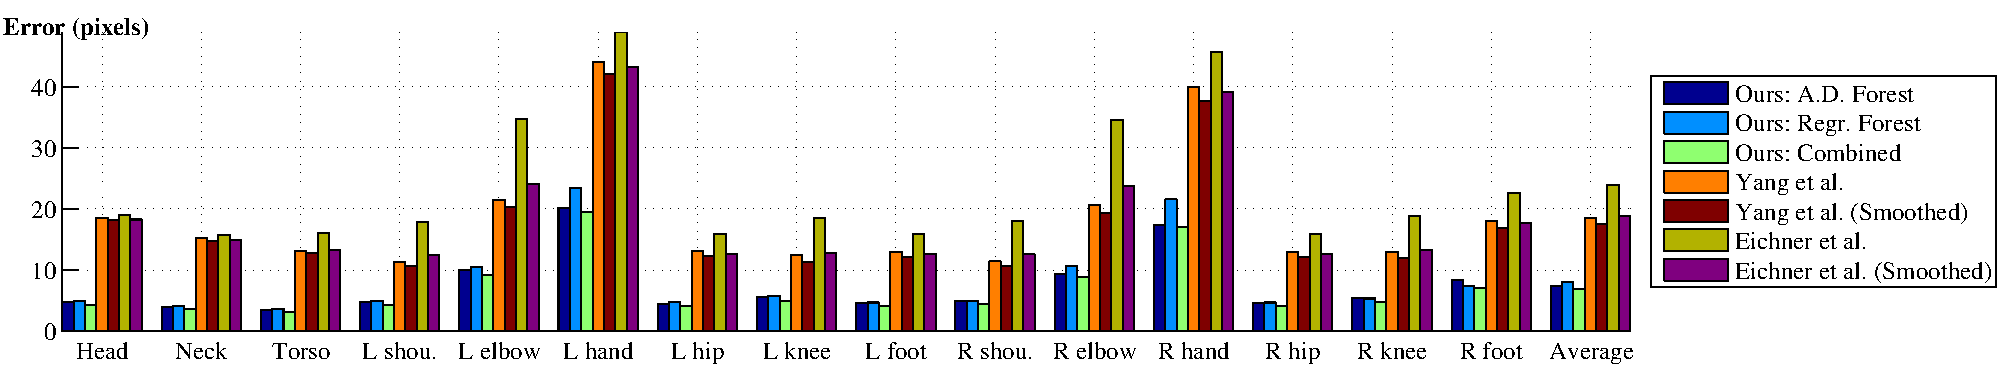
\includegraphics[width=1.02\linewidth]{fig/body/errplot2d.pdf} 
 	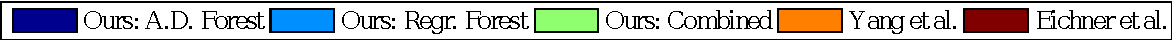
\includegraphics[width=0.6\linewidth]{fig/body/plot_legend.pdf}
	\caption{2D joint localisation errors of our methods, \cite{Yang2011} and \cite{Eichner2012} their median smoothed versions.}
\label{fig/body/errorplot2d}
\end{figure} 

\section{Evaluation}
\label{sec/body/evaluation}

\subsection{The APE Evaluation Dataset}
Experiments were performed to investigate the feasibility of the proposed approach. 
Existing public 3D pose datasets are inadequate to justify the main objectives of the proposed approach. Whilst benchmarks such as \cite{Sigal2010, Yao2012} model joint angles rather than joint positions using sophisticated techniques, e.g. camera networks, from a static area, our framework focuses on flexible, multi-action 3D HPE from monocular videos without using background statistics.

To this end, we collected the \emph{action-pose-estimation (APE)} dataset for both quantitative and qualitative evaluations. The APE dataset contains $245$ sequences from $7$ subjects performing $7$ categories of actions. Videos of each subject were recorded in different environments, changing camera poses and moving background objects. The APE dataset will be made publicly available. 
%We refer the reader to \cite{APEwebsite} for details about the dataset.

The setting of APE dataset is considered challenging for traditional 3D HPE because: (1) no scene-dependent cues, \eg foreground segmentation, can be applied, (2) testing is done in unseen environments. 
Experiments are divided into two parts. In the first part, pose estimation accuracy was evaluated quantitatively with ground truth and current state-of-the-arts, in 3D and 2D respectively. In the second part, we demonstrated the knowledge transfer ability qualitatively, by testing with other videos and datasets.     


\subsection{Experimental Results}

\begin{figure}[ht]
\centering
	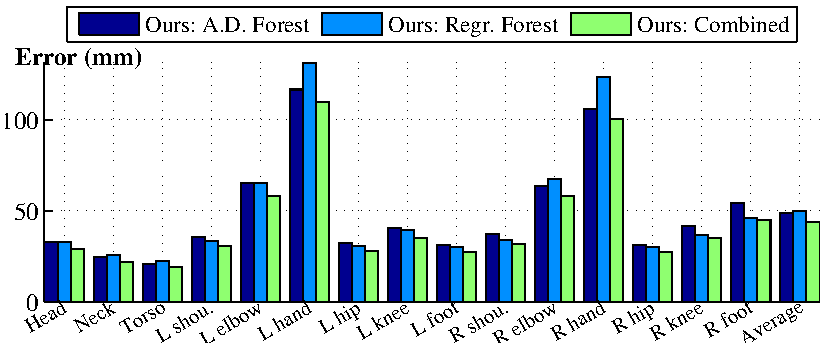
\includegraphics[width=0.8\linewidth]{fig/body/errplot3d.pdf} 
	\caption{3D joint localisation errors based on ground truth pose from Kinect sensor}
\label{fig/body/errorplot3d}
\end{figure}



\begin{figure}[ht]
	\centering
	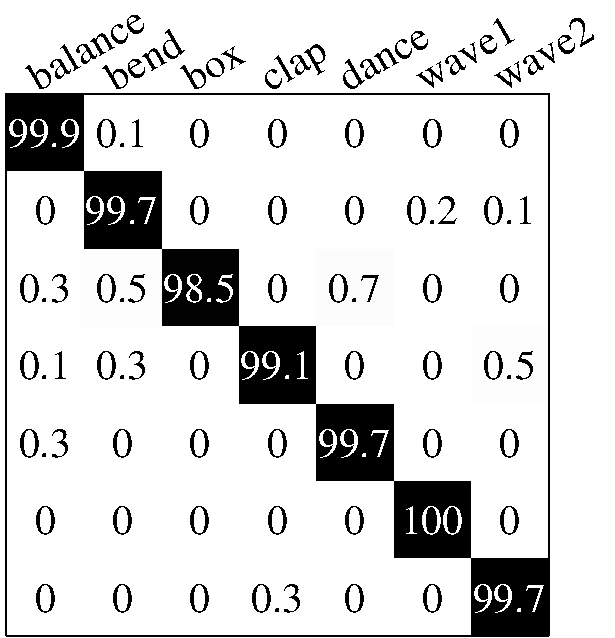
\includegraphics[height=0.30\linewidth]{fig/body/confm_detection.pdf} \hspace{1cm} 
	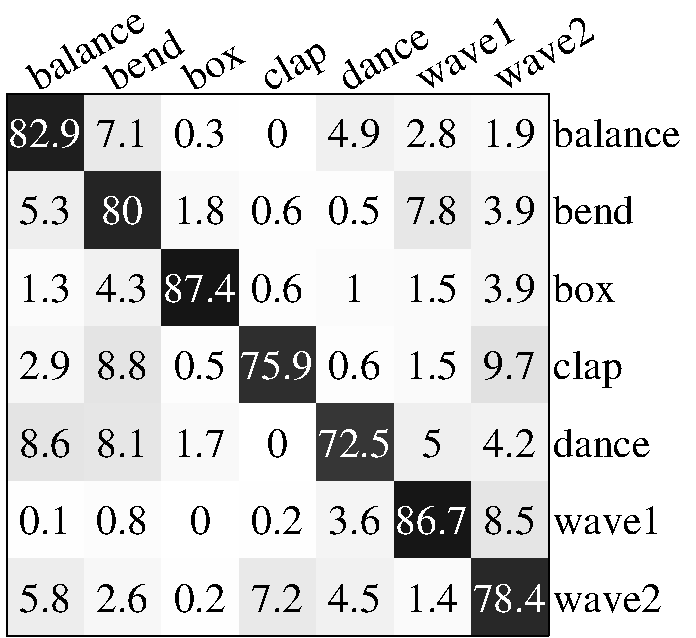
\includegraphics[height=0.30\linewidth]{fig/body/confm_regression.pdf}
	\caption{Confusion matrices of action classification by (left) action detection forest, and (right) cross-modality regression forest} 
	\label{fig/body/confm}
\end{figure}

\paragraph{Quantitative Evaluation.}
\label{sec/body/quant}
The proposed approach was evaluated quantitatively using the leave-one-out cross-validation strategy. A subject was taken out in turn for testing, thus the model is trained with $210$ sequences and the remaining $35$ sequences are evaluated. 
Snippets are extracted densely from training and testing data, where $\snippetlen = 10$. 
Table \ref{tab/body/rf_train_params} lists the training parameters. 
%Parameters used in training are shown in table \ref{tab/body/rf_train_params}. 

\begin{table}
	\centering
	\begin{tabular}{|c|c|c|c|}
		\hline 
		Forest & \# tree & Max. depth & Min. node size \\ \hline 
		$\forestd$ & 10 & 16 & 15 \\ \hline 
		$\forestr$ & 10 & 14 & 20 \\ \hline 
	\end{tabular} 
	\caption{Parameters used in training $\forestd$ and $\forestr$.}
	\label{tab/body/rf_train_params}
\end{table}

\begin{table}[ht]
\centering
\begin{tabular}{|p{4.5cm}|c|c|c|c|c|c|c|}
\hline
\backslashbox[4.5cm]{\textbf{Method}}{\textbf{Action}} & 
\rotatebox{60}{\textbf{Balance}}
& 
\rotatebox{60}{\textbf{Bend}}
& 
\rotatebox{60}{\textbf{Box}}		
& 
\rotatebox{60}{\textbf{Clap}}	
&
\rotatebox{60}{\textbf{Dance}}
& 
\rotatebox{60}{\textbf{Wave 1}}
& 
\rotatebox{60}{\textbf{Wave 2}}
\\ 
\hline
\hline
Action detection forest  	& 41.9 			& \textbf{\color{blue}58.6} & 84.3 			& 49.1 			& 47.4 			& 36.7 			& 36.2 \\ 
Regression forest 	& 41.4 			& 69.7 			& \textbf{\color{blue}60.3} & 52.2 			& 58.2 			& 36.1 			& 39.1 \\ 
Combined & \textbf{\color{blue}37.8} & 58.8 			& 66.2 			& \textbf{\color{blue}41.0} & \textbf{\color{blue}45.1} & \textbf{\color{blue}30.1} & \textbf{\color{blue}34.6}\\  
\hline
\end{tabular}
\caption{Per-class joint localisation accuracy (3D)} 
\label{tab/body/errperclass3D}
\end{table}


Pose estimation accuracy was evaluated in both 2D and 3D. Accuracies of 3D joint coordinates were compared directly with ground truth 3D poses captured by the Kinect sensor. Accuracies in 2D were measured by back-projecting the poses to image coordinates.  
Besides the combined pose estimation $\finalbodypose$, we also evaluated each of the forests alone, and compared it with the latest 2D HPE algorithms \cite{Eichner2012} and \cite{Yang2011}. 
In order to cope with actions performed in different speeds, testing videos are preprocessed by normalising with respect to their action speeds estimated from the first $25$ frames of the videos.
In order to make a fair comparison, the joint coordinates from the frame-based algorithms \cite{Eichner2012} and \cite{Yang2011} are temporally smoothed by a $10$-frame median filter, as our approach estimates poses from multiple-frame snippets. 

Action classification rates of individual frames by both forests are presented in figure \ref{fig/body/confm}. 
The action detection forest achieves excellent accuracy, as it has been optimised for classification during learning, the video-based input, snippet, also provides temporal cues that improve classification. It complements the regression forests that focus on the localisation accuracy of joints.    
The average 3D joint localisation errors of the experiments were reported in figure \ref{fig/body/errorplot3d}. 
Sample results of the proposed method are also presented in figures \ref{fig/body/APE1}, \ref{fig/body/APE2} and \ref{fig/body/APE3}. 

The comparison our method and other 2D HPE algorithms is illustrated in figure \ref{fig/body/errorplot2d}.
The proposed framework showed promising results, by extending the flexibility of \cite{Yang2011}, the proposed method showed high robustness in 3D pose estimation and outperformed both state-of-the-arts in the 2D tests. The hand parts have the highest localisation errors because of their large movements and frequent occlusions, which are as well indicated by the big variance ellipsoids in figures \ref{fig/body/APE1}, \ref{fig/body/APE2}, \ref{fig/body/APE3}.

The per-class localisation errors are listed in table \ref{tab/body/errperclass3D} (3D) and \ref{tab/body/errperclass2D} (2D). While some classes reported significant improvements after combining the results of action detection and pose regression, \eg ``clap'' and ``wave 1'', the ``bend'' and ``box'' class reported the highest error rates.
The 2D part detections obtained from the ``box'' and ``bend'' classes are less accurate than those from other classes.  For the ``box'' action, self-occlusion happens frequently such that the part detector is confused about the left and right hand positions, making the hand position distributions spread around the torso as in figure \ref{fig/body/APEerr2} and \ref{fig/body/APEerr3}. 
Similarly, when the arms are stretched overhead and occluded, the 2D DPM model used in the experiments gives incorrect results.  

% classnames = {'wave2','balance','bend','box','clap','dance','wave1'};
\begin{figure}
	\centering 
	\begin{subfigure}[b]{1\linewidth}
		\centering
		\begin{tabular}{c|cccc}
			\raisebox{1cm}{\textbf{Input}} &
			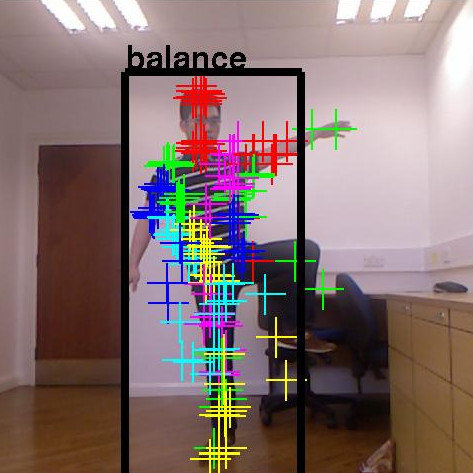
\includegraphics[height=2.3cm]{fig/body/APE/balc1.jpg} & 
			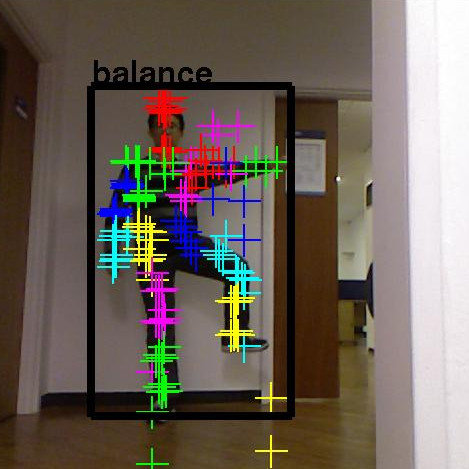
\includegraphics[height=2.3cm]{fig/body/APE/balc2.jpg} &
			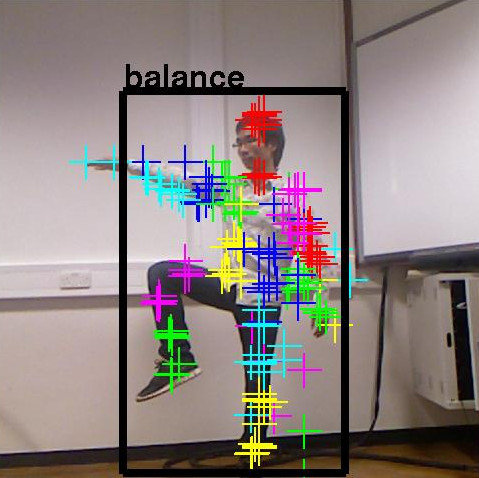
\includegraphics[height=2.3cm]{fig/body/APE/balc3.jpg} & 
			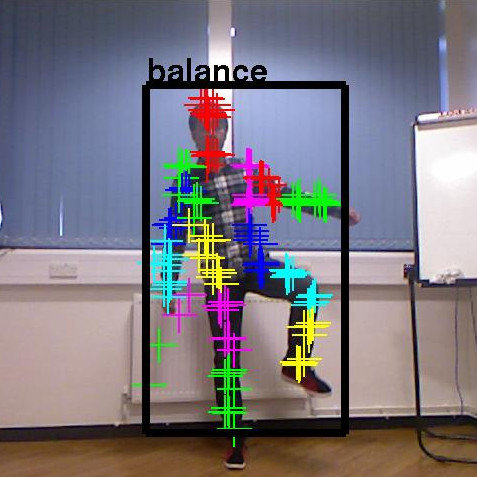
\includegraphics[height=2.3cm]{fig/body/APE/balc4.jpg} \\
			\raisebox{1cm}{\textbf{3D pose}} &
			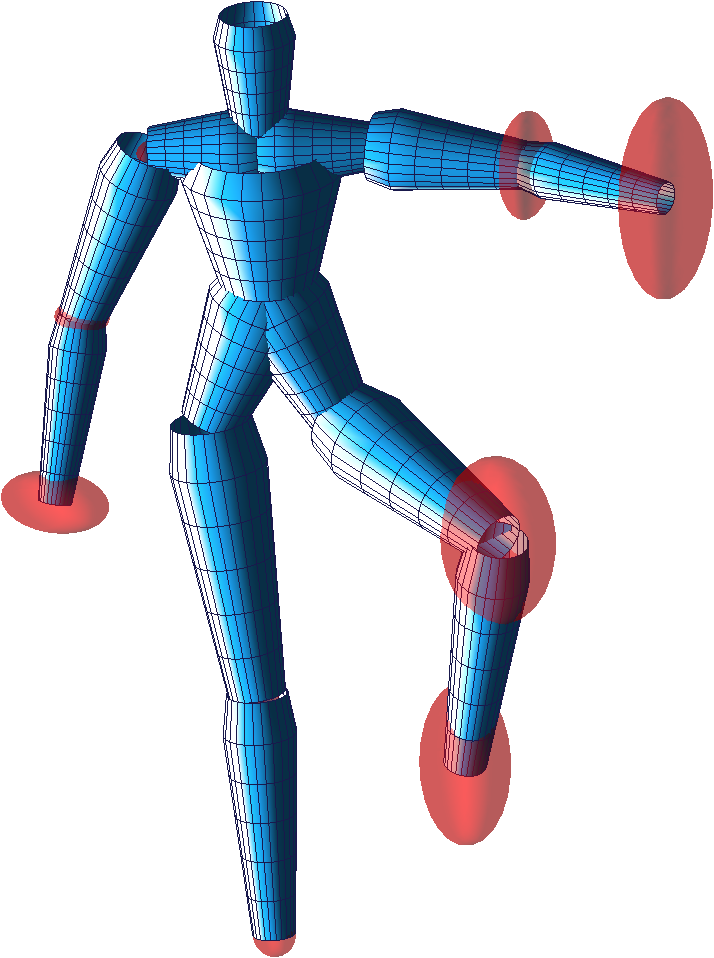
\includegraphics[height=2.3cm]{fig/body/APE/balc1.png} & 
			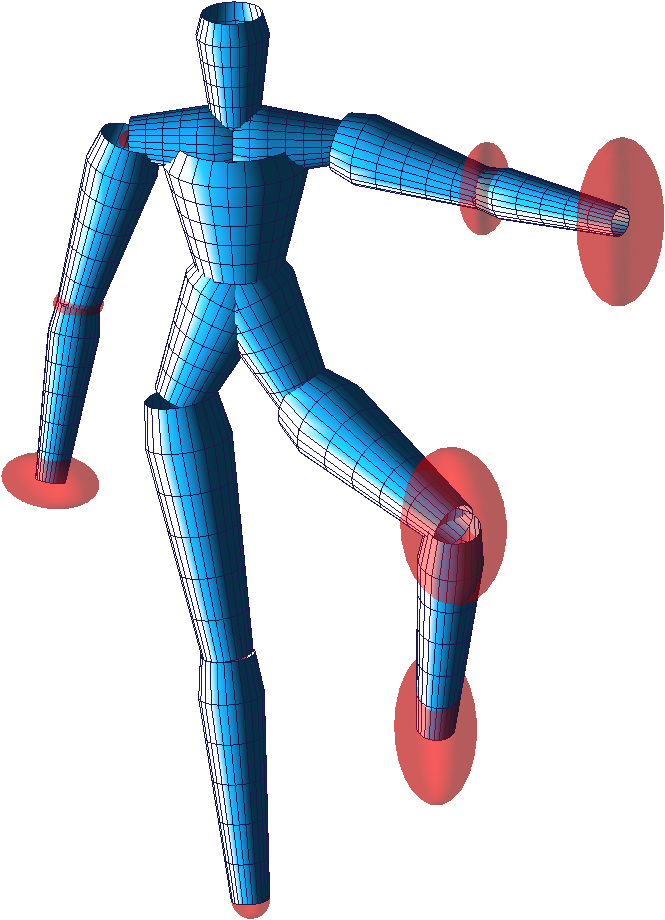
\includegraphics[height=2.3cm]{fig/body/APE/balc2.png} &
			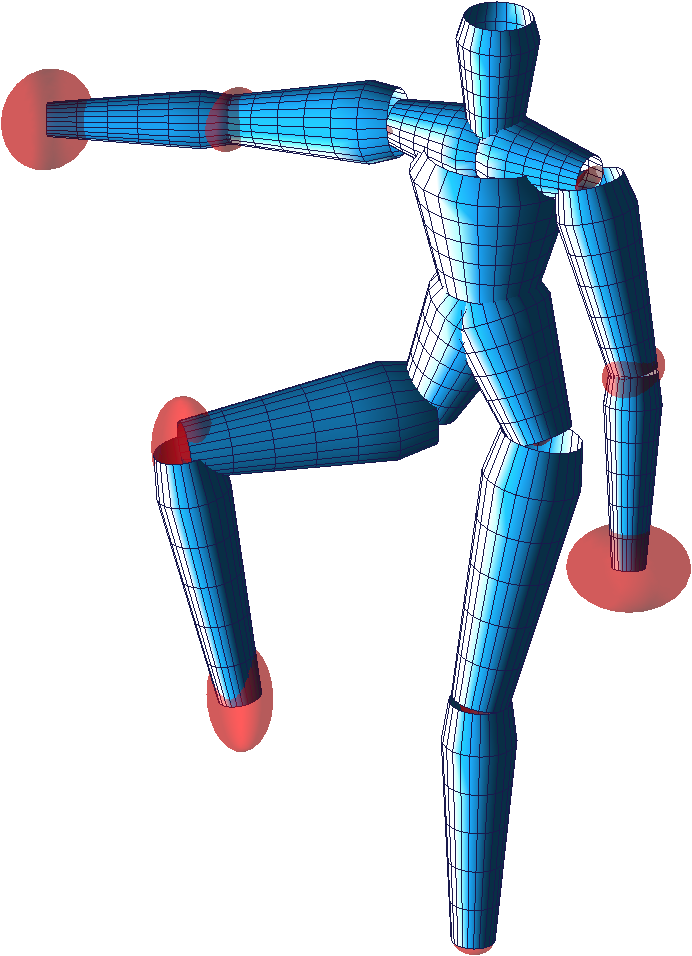
\includegraphics[height=2.3cm]{fig/body/APE/balc3.png} & 
			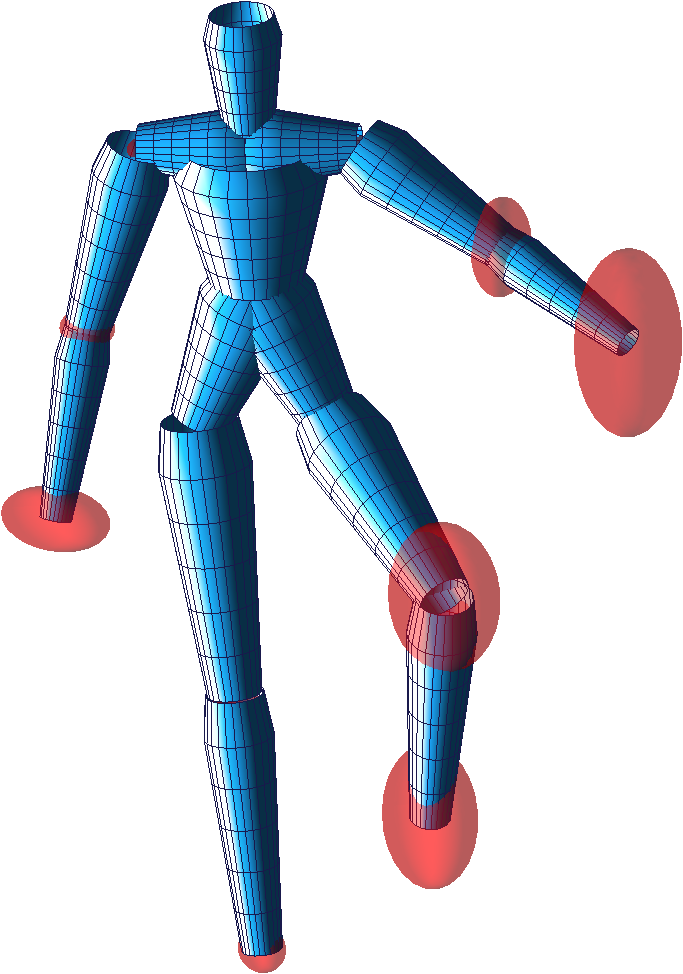
\includegraphics[height=2.3cm]{fig/body/APE/balc4.png} 
		\end{tabular}
		\subcaption{Balance}
		\label{fig/body/APE/balc} 
	\end{subfigure}
	\begin{subfigure}[b]{1\linewidth}
		\centering
		\begin{tabular}{c|cccc}
			\raisebox{1cm}{\textbf{Input}} &
			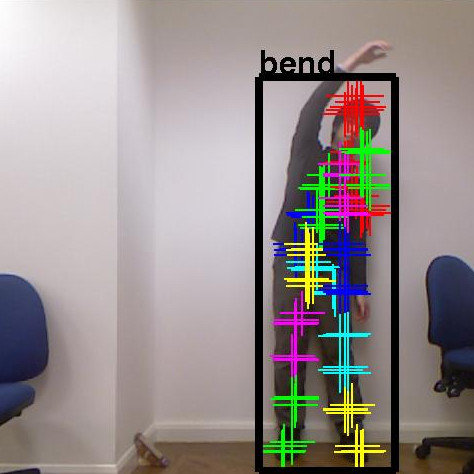
\includegraphics[height=2.3cm]{fig/body/APE/bend1.jpg} & 
			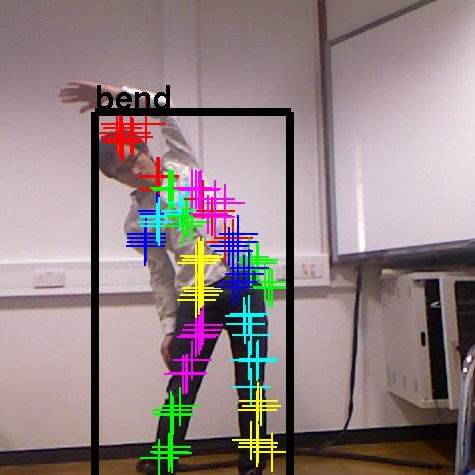
\includegraphics[height=2.3cm]{fig/body/APE/bend2.jpg} &
			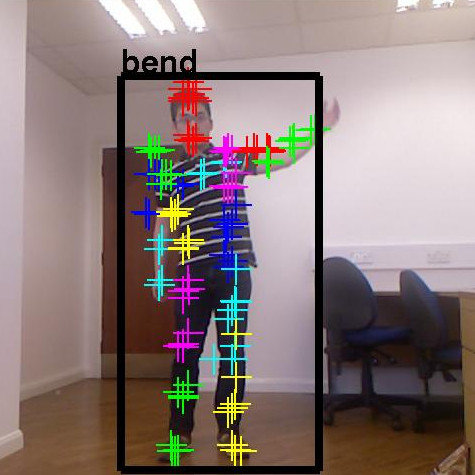
\includegraphics[height=2.3cm]{fig/body/APE/bend3.jpg} & 
			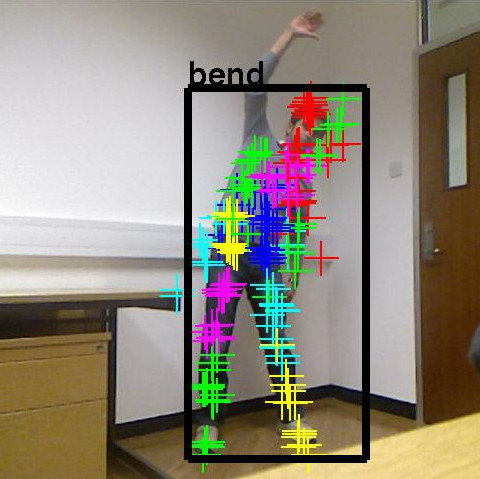
\includegraphics[height=2.3cm]{fig/body/APE/bend4.jpg} \\
			\raisebox{1cm}{\textbf{3D pose}} &
			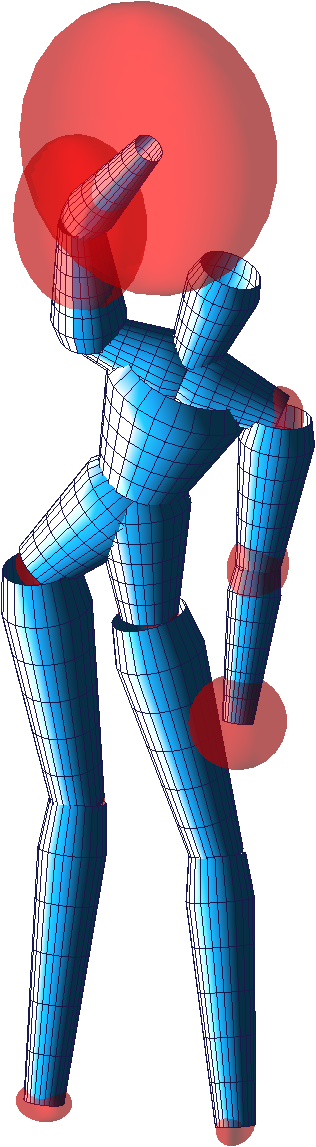
\includegraphics[height=2.3cm]{fig/body/APE/bend1.png} & 
			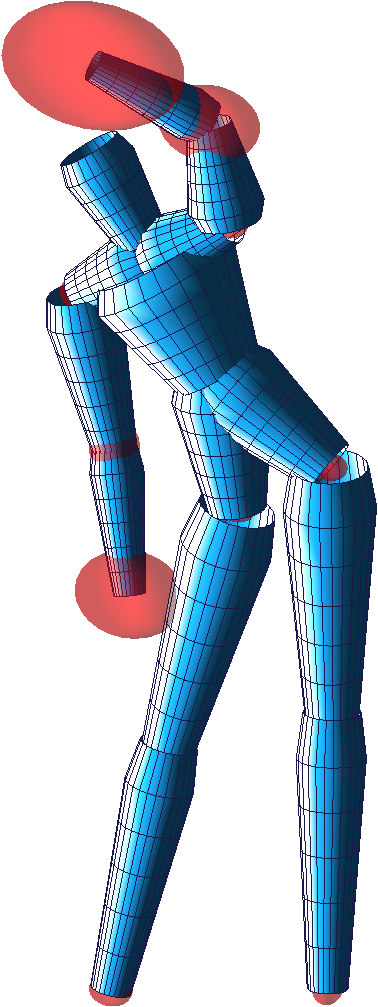
\includegraphics[height=2.3cm]{fig/body/APE/bend2.png} &
			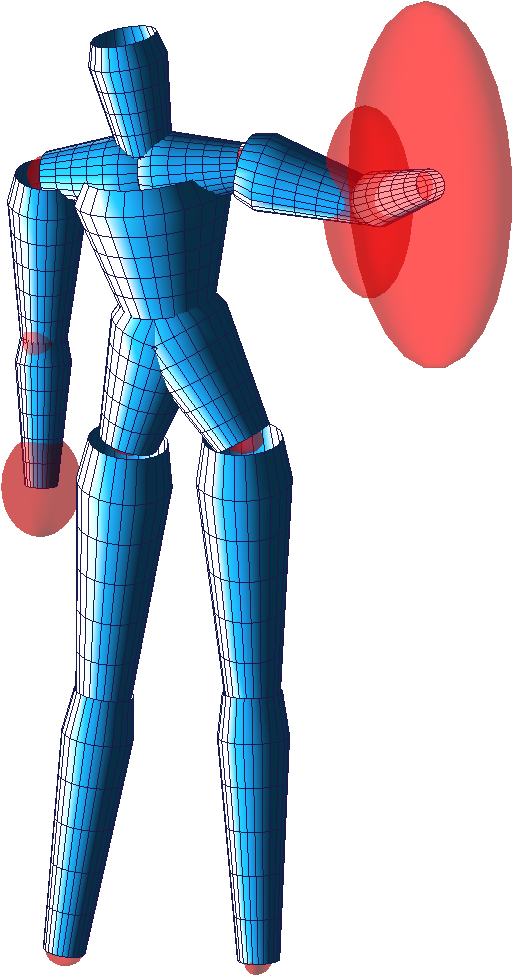
\includegraphics[height=2.3cm]{fig/body/APE/bend3.png} & 
			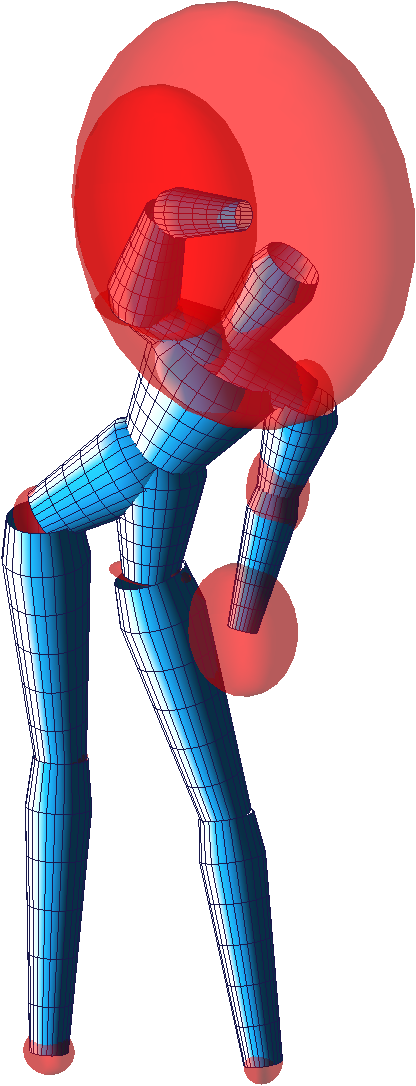
\includegraphics[height=2.3cm]{fig/body/APE/bend4.png} 
		\end{tabular}
		\subcaption{Bend}
		\label{fig/body/APE/bend} 
	\end{subfigure}
	\begin{subfigure}[b]{1\linewidth}
		\centering
		\begin{tabular}{c|cccc}
			\raisebox{1cm}{\textbf{Input}} &
			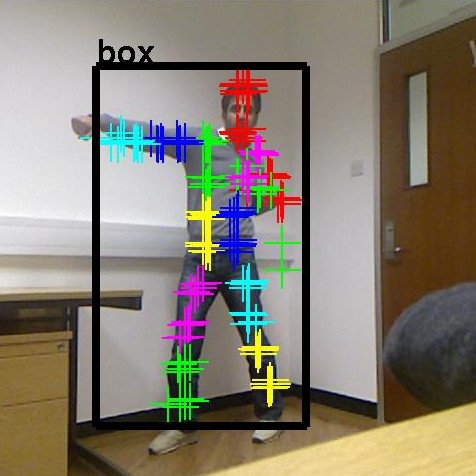
\includegraphics[height=2.3cm]{fig/body/APE/boxx1.jpg} & 
			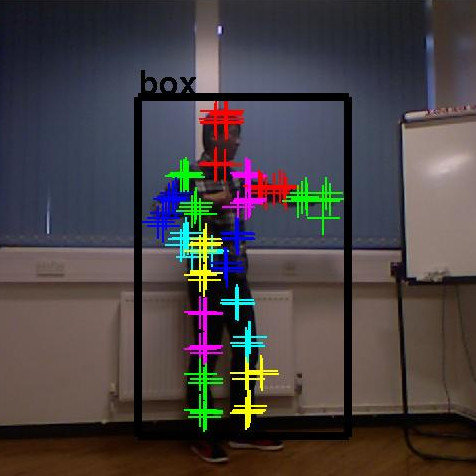
\includegraphics[height=2.3cm]{fig/body/APE/boxx2.jpg} &
			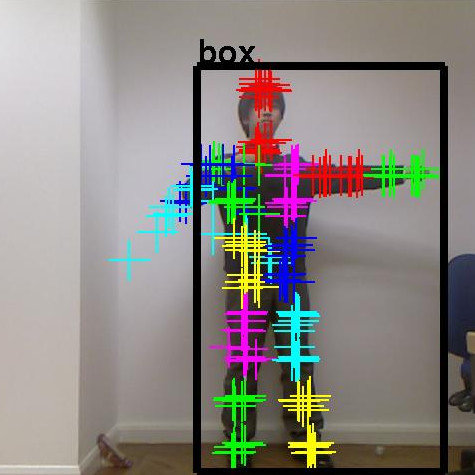
\includegraphics[height=2.3cm]{fig/body/APE/boxx3.jpg} & 
			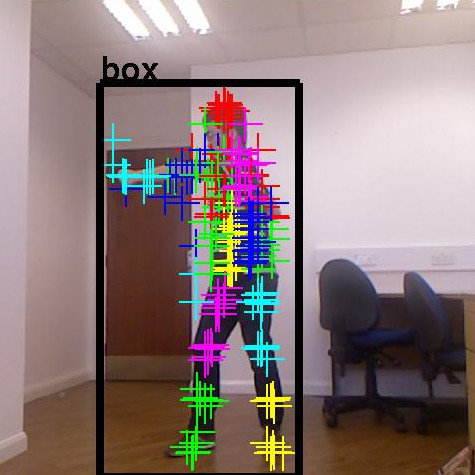
\includegraphics[height=2.3cm]{fig/body/APE/boxx4.jpg} \\
			\raisebox{1cm}{\textbf{3D pose}} &
			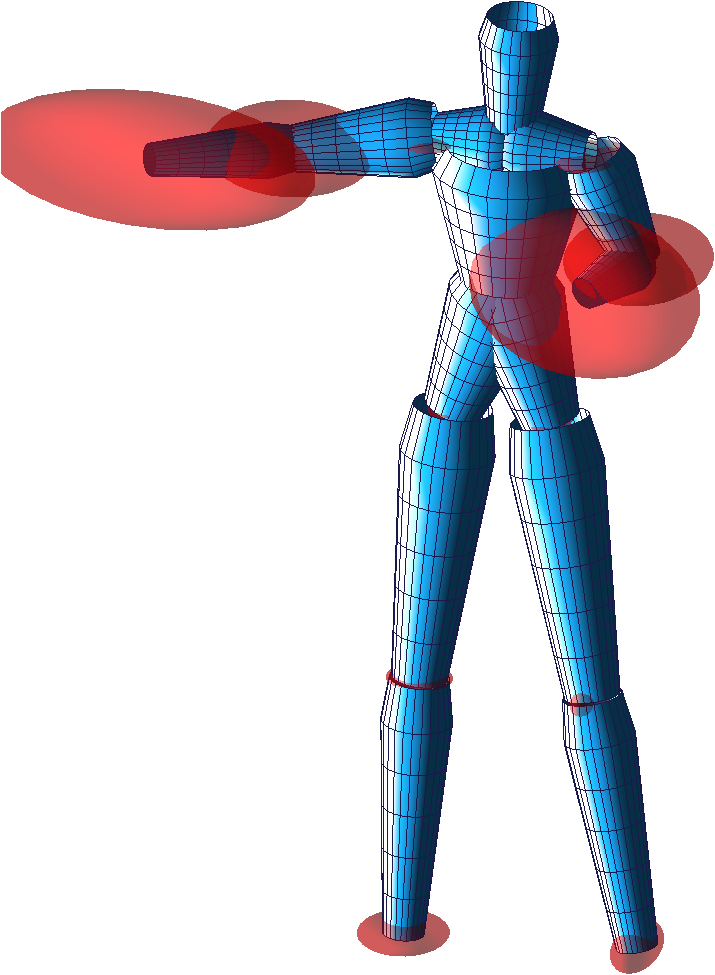
\includegraphics[height=2.3cm]{fig/body/APE/boxx1.png} & 
			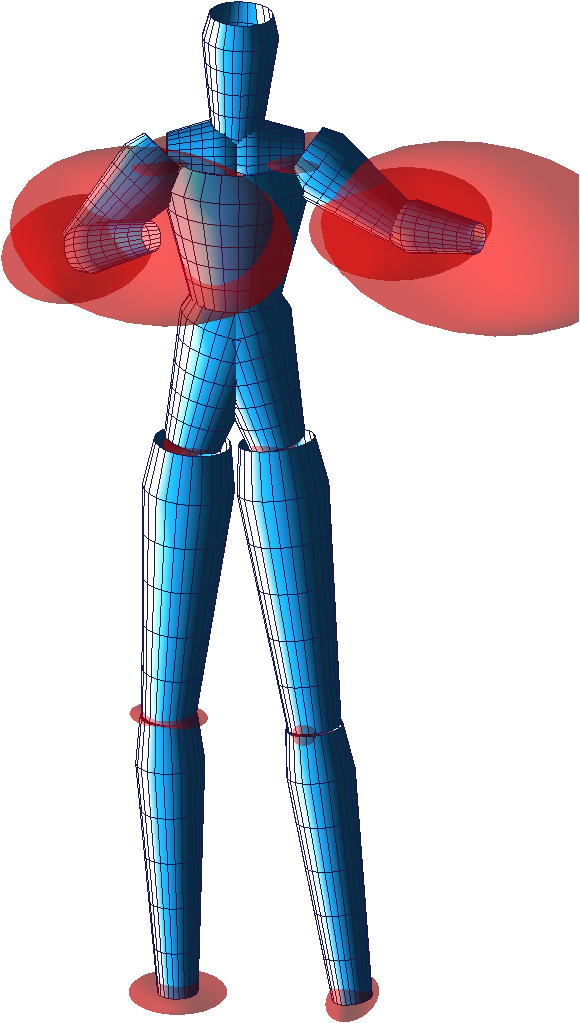
\includegraphics[height=2.3cm]{fig/body/APE/boxx2.png} &
			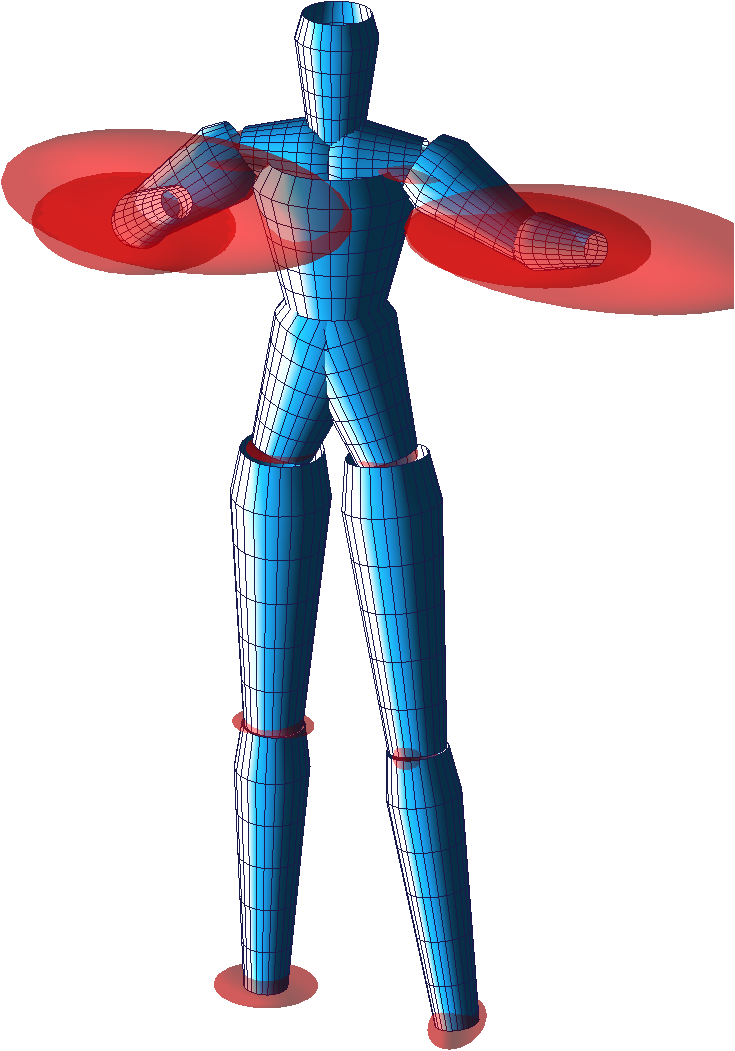
\includegraphics[height=2.3cm]{fig/body/APE/boxx3.png} & 
			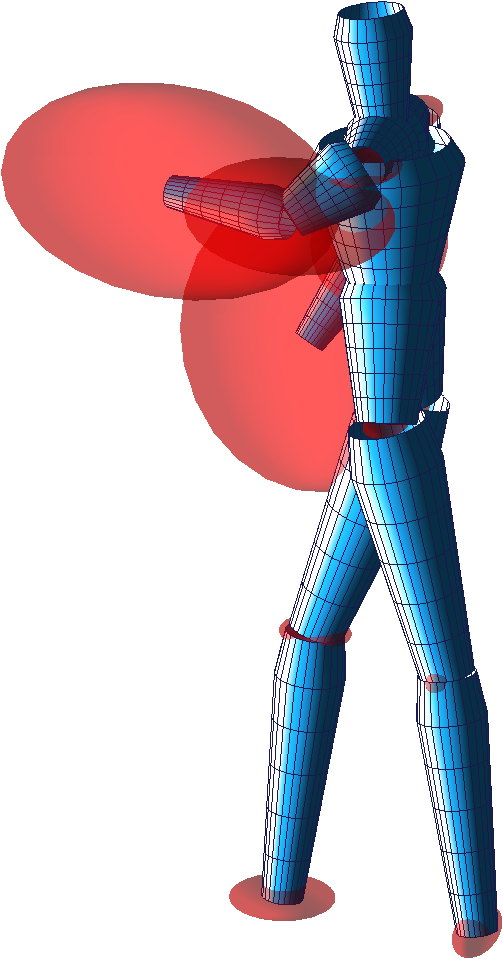
\includegraphics[height=2.3cm]{fig/body/APE/boxx4.png} 
		\end{tabular}
		\subcaption{Box}
		\label{fig/body/APE/boxx} 
	\end{subfigure}
	\caption{\textbf{3-D pose estimation results of the APE dataset.} From top to bottom: (a) balance, (b) bend, and (c) box.}
	\label{fig/body/APE1}
\end{figure}

\begin{figure}
	\centering 
	\begin{subfigure}[b]{1\linewidth}
		\centering
		\begin{tabular}{c|cccc}
			\raisebox{1cm}{\textbf{Input}} &
			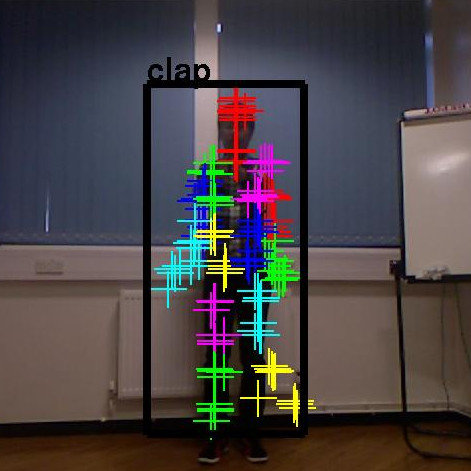
\includegraphics[height=2.3cm]{fig/body/APE/clap1.jpg} & 
			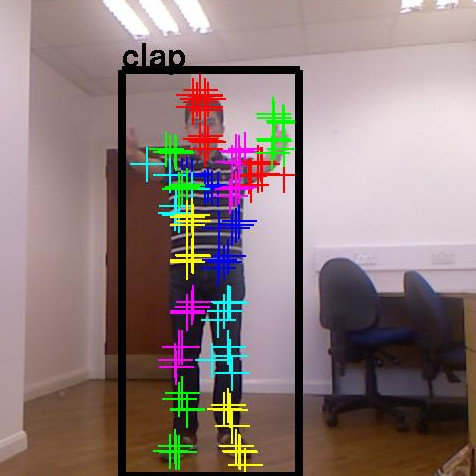
\includegraphics[height=2.3cm]{fig/body/APE/clap2.jpg} &
			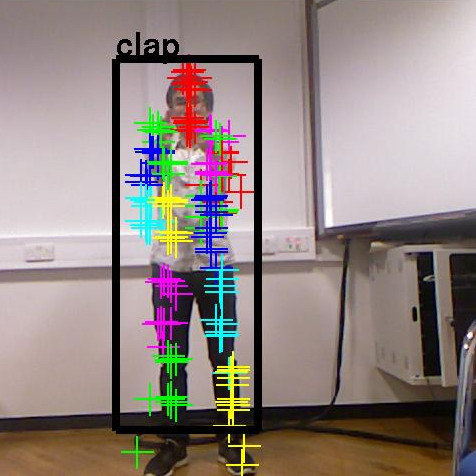
\includegraphics[height=2.3cm]{fig/body/APE/clap3.jpg} & 
			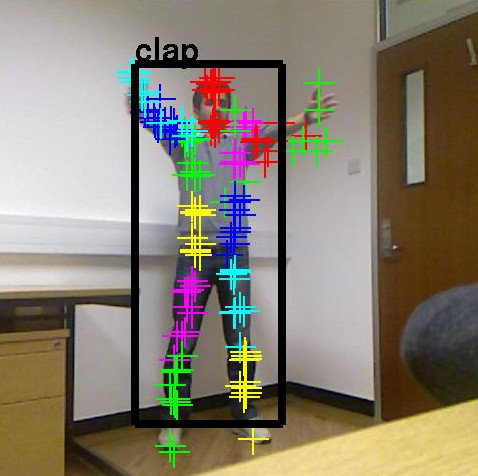
\includegraphics[height=2.3cm]{fig/body/APE/clap4.jpg} \\
			\raisebox{1cm}{\textbf{3D pose}} &
			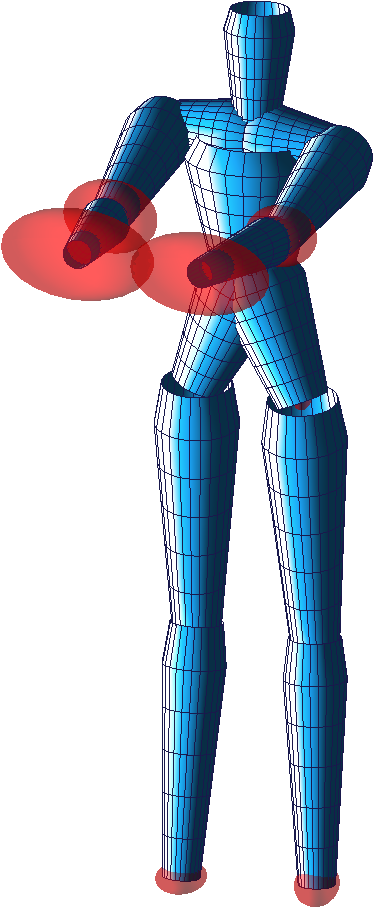
\includegraphics[height=2.3cm]{fig/body/APE/clap1.png} & 
			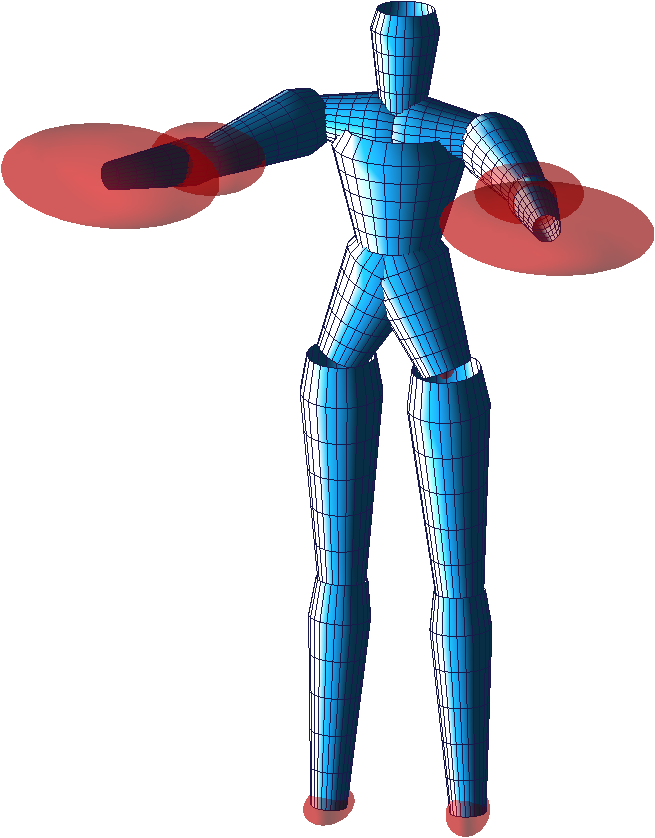
\includegraphics[height=2.3cm]{fig/body/APE/clap2.png} &
			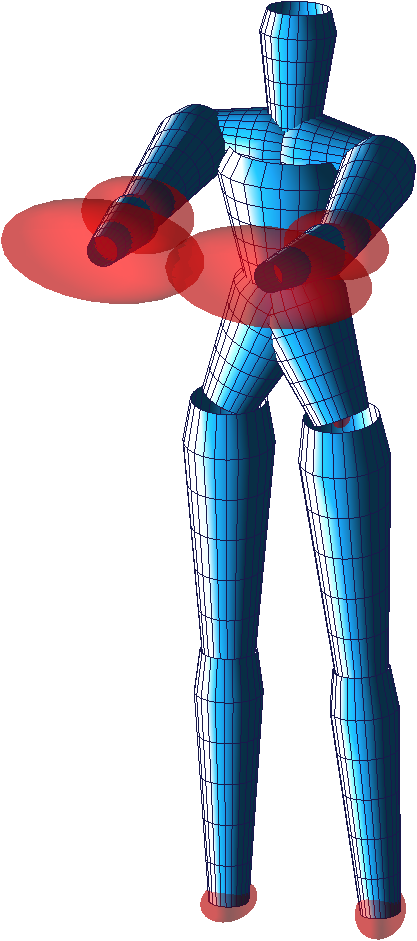
\includegraphics[height=2.3cm]{fig/body/APE/clap3.png} & 
			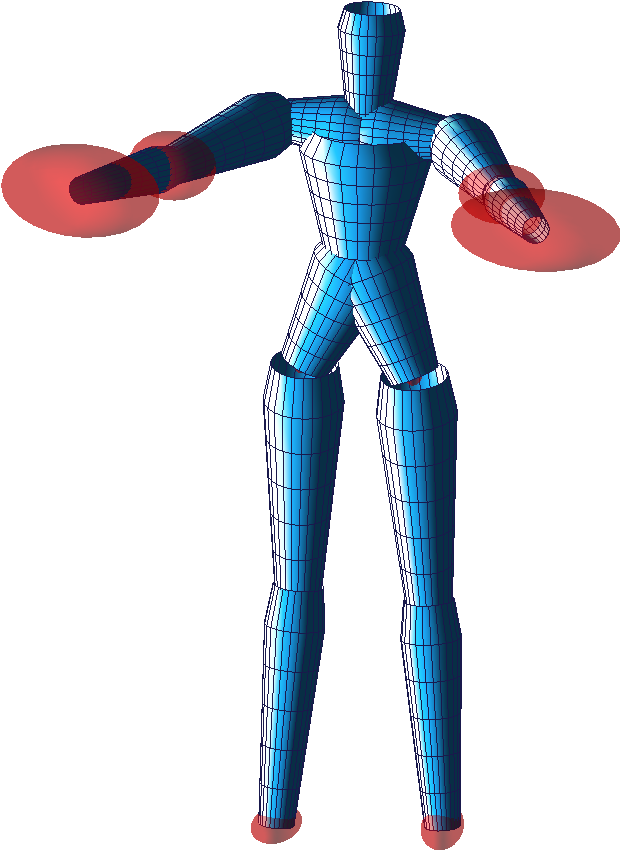
\includegraphics[height=2.3cm]{fig/body/APE/clap4.png} 
		\end{tabular}
		\subcaption{Clap}
		\label{fig/body/APE/clap} 
	\end{subfigure}
	\begin{subfigure}[b]{1\linewidth}
		\centering
		\begin{tabular}{c|cccc}
			\raisebox{1cm}{\textbf{Input}} &
			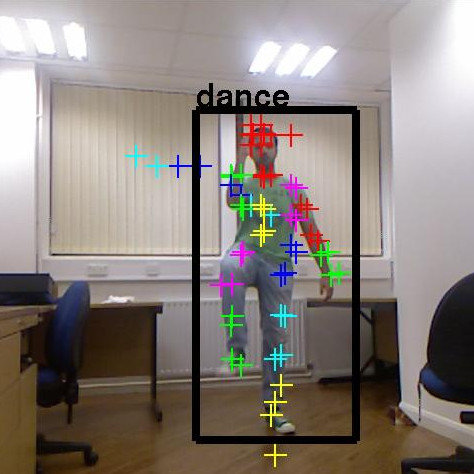
\includegraphics[height=2.3cm]{fig/body/APE/dance1.jpg} & 
			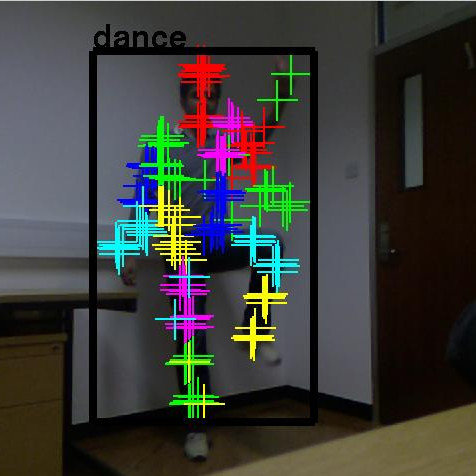
\includegraphics[height=2.3cm]{fig/body/APE/dance2.jpg} &
			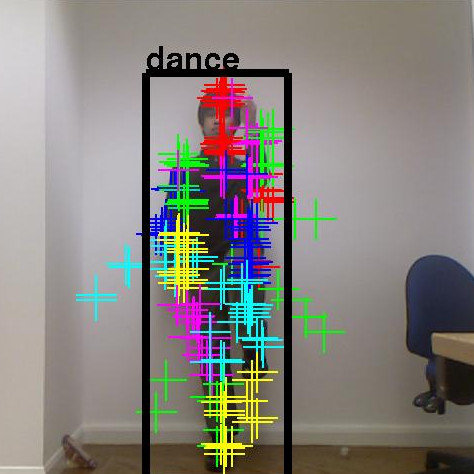
\includegraphics[height=2.3cm]{fig/body/APE/dance3.jpg} & 
			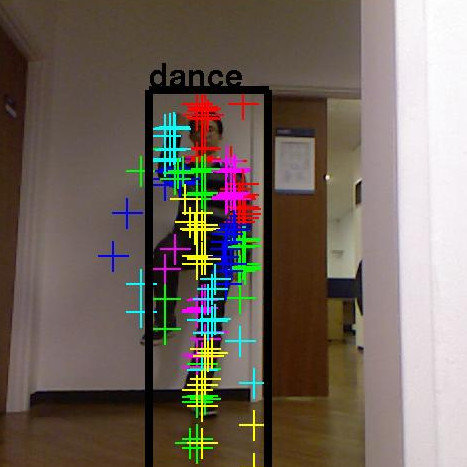
\includegraphics[height=2.3cm]{fig/body/APE/dance4.jpg} \\
			\raisebox{1cm}{\textbf{3D pose}} &
			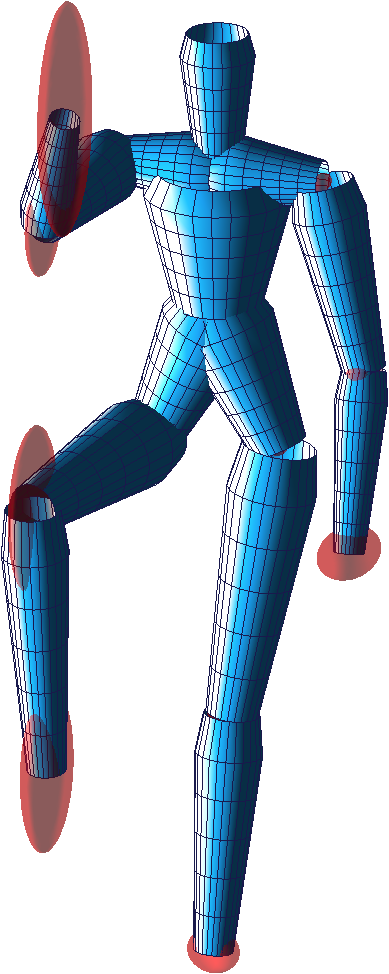
\includegraphics[height=2.3cm]{fig/body/APE/dance1.png} & 
			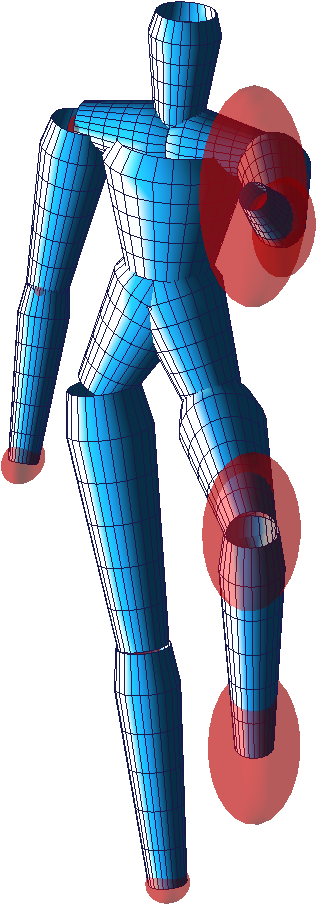
\includegraphics[height=2.3cm]{fig/body/APE/dance2.png} &
			\includegraphics[height=2.3cm]{fig/body/APE/dance3.png} & 
			\includegraphics[height=2.3cm]{fig/body/APE/dance4.png} 
		\end{tabular}
		\subcaption{Dance}
		\label{fig/body/APE/dance} 
	\end{subfigure}
	\begin{subfigure}[b]{1\linewidth}
		\centering
		\begin{tabular}{c|cccc}
			\raisebox{1cm}{\textbf{Input}} &
			\includegraphics[height=2.3cm]{fig/body/APE/wave11.jpg} & 
			\includegraphics[height=2.3cm]{fig/body/APE/wave12.jpg} &
			\includegraphics[height=2.3cm]{fig/body/APE/wave13.jpg} & 
			\includegraphics[height=2.3cm]{fig/body/APE/wave14.jpg} \\
			\raisebox{1cm}{\textbf{3D pose}} &
			\includegraphics[height=2.3cm]{fig/body/APE/wave11.png} & 
			\includegraphics[height=2.3cm]{fig/body/APE/wave12.png} &
			\includegraphics[height=2.3cm]{fig/body/APE/wave13.png} & 
			\includegraphics[height=2.3cm]{fig/body/APE/wave14.png} 
		\end{tabular}
		\subcaption{Wave 1}
		\label{fig/body/APE/wave1} 
	\end{subfigure}
	\caption{\textbf{3-D pose estimation results of APE dataset.} From top to bottom: (a) clap, (b) dance, and (c) wave 1}
	\label{fig/body/APE2}
\end{figure}

\begin{figure}
	\centering 
	\begin{tabular}{c|cccc}
		\raisebox{1cm}{\textbf{Input}} &
		\includegraphics[height=2.3cm]{fig/body/APE/wave21.jpg} & 
		\includegraphics[height=2.3cm]{fig/body/APE/wave22.jpg} &
		\includegraphics[height=2.3cm]{fig/body/APE/wave23.jpg} & 
		\includegraphics[height=2.3cm]{fig/body/APE/wave24.jpg} \\
		\raisebox{1cm}{\textbf{3D pose}} &
		\includegraphics[height=2.3cm]{fig/body/APE/wave21.png} & 
		\includegraphics[height=2.3cm]{fig/body/APE/wave22.png} &
		\includegraphics[height=2.3cm]{fig/body/APE/wave23.png} & 
		\includegraphics[height=2.3cm]{fig/body/APE/wave24.png} 
	\end{tabular}
	\label{fig/body/APE/wave2} 
	\caption{\textbf{3-D pose estimation results of the ``wave 2'' action class.}}
	\label{fig/body/APE3}
\end{figure}

\begin{figure}
	\centering 
	\begin{tabular}{c}
		\raisebox{-0.3cm}{\textbf{Input}} \\ 
		\raisebox{-2.1cm}{\textbf{3D pose}}
	\end{tabular} 
	\begin{tabular}{c|}
		\vbox to 4.6cm {\vfil
			\hbox to 1mm{}%
			\vfil
		}
	\end{tabular}
	\begin{subfigure}[t]{0.18\linewidth} \centering
		\includegraphics[height=2.3cm]{fig/body/APE/benderr.jpg} \\
		\includegraphics[height=2.3cm]{fig/body/APE/benderr.png} 
		\subcaption{Bend}
		\label{fig/body/APEerr1}
	\end{subfigure}
	\begin{subfigure}[t]{0.18\linewidth} \centering
		\includegraphics[height=2.3cm]{fig/body/APE/boxxerr.jpg} \\
		\includegraphics[height=2.3cm]{fig/body/APE/boxxerr.png} 
		\subcaption{Box}
		\label{fig/body/APEerr2}
	\end{subfigure}
	\begin{subfigure}[t]{0.18\linewidth} \centering
		\includegraphics[height=2.3cm]{fig/body/APE/boxerr2.jpg} \\
		\includegraphics[height=2.3cm]{fig/body/APE/boxerr2.png} 
		\subcaption{Box}
		\label{fig/body/APEerr3}
	\end{subfigure}
	\begin{subfigure}[t]{0.18\linewidth} \centering
		\includegraphics[height=2.3cm]{fig/body/APE/wave1err.jpg} \\
		\includegraphics[height=2.3cm]{fig/body/APE/wave1err.png} 
		\subcaption{Wave 1}
		\label{fig/body/APEerr4}
	\end{subfigure}
	\label{fig/body/APEerr}
	\caption{\textbf{Incorrect cases of 3-D pose estimation.}}
\end{figure}


\paragraph{Qualitative Evaluation.}
Knowledge transfer was evaluated by reusing the models trained in section \ref{sec/body/quant} to other datasets without retraining.
The KTH \cite{Schuldt2004} and Weizmann \cite{Gorelick2007} dataset were used in the experiments as they shared action categories with the APE dataset. 

The experimental results are reported qualitatively in figure \ref{fig/body/otherresults}. Even though the input videos are of extremely low resolutions, rendering them inapplicable to typical 3D HPE methods, our framework is still able to estimate their actions and poses simultaneously with encouraging accuracy. 
Incorrect poses were estimated when too many false positive parts are detected from the low resolution images, \eg figure \ref{fig/body/otherresults}(g--h). 

\paragraph{Discussion.}
The experimental results have demonstrated high feasibility in the idea of using action detection to estimate 3D poses under challenging conditions.  
Coupling the outputs from the random forests, the 3D pose estimation accuracy is further enhanced. Action detection gives a global pose estimation and the corresponding class label. Meanwhile, errors in the initial global estimation, due to the differences among individual action patterns, are corrected locally by regression forests, which improves the accuracy of the final pose estimation as shown in figure \ref{fig/body/errorplot3d}. 

On the other side, there is still room for improvement in the proposed approach. The proposed method relies on DPM as the only source of input. Albeit great flexibility, \cf \cite{Yang2011}, the performance of a DPM depends on its training data. Our method handles minor errors gracefully by allowing multiple hypotheses and snippet-based input, but large errors cannot be recovered completely, \eg figure \ref{fig/body/APEerr1} and \ref{fig/body/APEerr2} for APE dataset, and \ref{fig/body/others/g} and \ref{fig/body/others/h} for KTH and Weizmann dataset respectively. 
Besides, the proposed method runs at $0.31$fps. Feature extraction from DPM is the run-time bottleneck. The pose estimatior alone runs at about $5$fps by precomputing the DPM features. 

\begin{figure}
	\centering 
	\begin{tabular}{c}
		\raisebox{-0.3cm}{\textbf{Input}} \\ 
		\raisebox{-2.1cm}{\textbf{3D pose}}
	\end{tabular} 
	\begin{tabular}{c|}
		\vbox to 4.6cm {\vfil
			\hbox to 1mm{}%
			\vfil
		}
	\end{tabular}
	\begin{subfigure}[t]{0.18\linewidth} \centering
		\includegraphics[height=2.3cm]{fig/body/others/kth3.jpg} \\
		\includegraphics[height=2.3cm]{fig/body/others/kth3.png} 
		\subcaption{Wave 2}
		\label{fig/body/others/a}
	\end{subfigure}
	\begin{subfigure}[t]{0.18\linewidth} \centering
		\includegraphics[height=2.3cm]{fig/body/others/kth1.jpg} \\
		\includegraphics[height=2.3cm]{fig/body/others/kth1.png} 
		\subcaption{Wave 2}
		\label{fig/body/others/b}
	\end{subfigure}
	\begin{subfigure}[t]{0.18\linewidth} \centering
		\includegraphics[height=2.3cm]{fig/body/others/kth2.jpg} \\
		\includegraphics[height=2.3cm]{fig/body/others/kth2.png} 
		\subcaption{Clap}
		\label{fig/body/others/c}
	\end{subfigure}
	\begin{subfigure}[t]{0.18\linewidth} \centering
		\includegraphics[height=2.3cm]{fig/body/others/weiz3.jpg} \\
		\includegraphics[height=2.3cm]{fig/body/others/weiz3.png} 
		\subcaption{Wave 1}
		\label{fig/body/others/d}
	\end{subfigure} \\ 
	\begin{tabular}{c}
		\raisebox{-0.3cm}{\textbf{Input}} \\ 
		\raisebox{-2.1cm}{\textbf{3D pose}}
	\end{tabular} 
	\begin{tabular}{c|}
		\vbox to 4.6cm {\vfil
			\hbox to 1mm{}%
			\vfil
		}
	\end{tabular}
	\begin{subfigure}[t]{0.18\linewidth} \centering
		\includegraphics[height=2.3cm]{fig/body/others/weiz1.jpg} \\
		\includegraphics[height=2.3cm]{fig/body/others/weiz1.png} 
		\subcaption{Wave 1}
		\label{fig/body/others/e}
	\end{subfigure}
	\begin{subfigure}[t]{0.18\linewidth} \centering
		\includegraphics[height=2.3cm]{fig/body/others/weiz2.jpg} \\
		\includegraphics[height=2.3cm]{fig/body/others/weiz2.png} 
		\subcaption{Wave 2}
		\label{fig/body/others/f}
	\end{subfigure}
	\begin{subfigure}[t]{0.18\linewidth} \centering
		\includegraphics[height=2.3cm]{fig/body/others/ktherr.jpg} \\
		\includegraphics[height=2.3cm]{fig/body/others/ktherr.png} 
		\subcaption{Wave 2}
		\label{fig/body/others/g}
	\end{subfigure}
	\begin{subfigure}[t]{0.18\linewidth} \centering
		\includegraphics[height=2.3cm]{fig/body/others/weizerr.jpg} \\
		\includegraphics[height=2.3cm]{fig/body/others/weizerr.png} 
		\subcaption{Wave 1}
		\label{fig/body/others/h}
	\end{subfigure}
	\caption{Sample results obtained from applying the model trained from APE dataset to KTH (a--c, g) and Weizmann dataset (d--f, h)} 
	\label{fig/body/otherresults}
\end{figure}



\section{Discussion}
\label{sec/body/conclusions}

The challenging problem of 3D human pose estimation is discussed in this chapter. 
While traditional methods for 3D human pose estimation emphasise accuracy over their compatibility with realistic applications, we present a novel practical approach without using any scene-dependent constraints.
We investigate the new area of using action for pose estimation. The proposed method combines human action detection and deformable part model-based 2D human pose estimation to estimate 3D poses from unconstrained, monocular videos.  
The new APE dataset is introduced to evaluate the feasibility of our approach.  
Experimental results have shown promising results and also high flexibility by transferring the knowledge obtained from training data to other unseen datasets.
In the future we plan to apply kinematic constraints in our system for pose refinement. 
We suggest that the collaboration between the techniques in human action and pose analysis will be beneficial to both areas of computer vision research in the coming future.  

